% ------------------------------------------------------------------------
% Ígor Assis Rocha Yamamoto
% contato@igoryamamoto.com
% Modelo criado a partir da abnTeX2, em conformes com a ABNT NBR 14724:2011
% ------------------------------------------------------------------------

\documentclass[
	% -- opções da classe memoir --
	12pt,				% tamanho da fonte
	openright,			% capítulos começam em pág ímpar (insere página vazia caso preciso)
	twoside,			% para impressão em verso e anverso. Oposto a oneside
	a4paper,			% tamanho do papel. 
	% -- opções da classe abntex2 --
	%chapter=TITLE,		% títulos de capítulos convertidos em letras maiúsculas
	%section=TITLE,		% títulos de seções convertidos em letras maiúsculas
	%subsection=TITLE,	% títulos de subseções convertidos em letras maiúsculas
	%subsubsection=TITLE,% títulos de subsubseções convertidos em letras maiúsculas
	% -- opções do pacote babel --
	english,			% idioma adicional para hifenização
	brazil				% o último idioma é o principal do documento
	]{abntex2}

% ---
% Pacotes básicos 
% ---
%\usepackage{arial}
\usepackage[T1]{fontenc}		% Selecao de codigos de fonte.
\usepackage[utf8]{inputenc}
\usepackage{lastpage}			% Usado pela Ficha catalográfica
\usepackage{indentfirst}		% Indenta o primeiro parágrafo de cada seção.
\usepackage{color}				% Controle das cores
\usepackage{graphicx}			% Inclusão de gráficos
\usepackage{microtype} 			% para melhorias de justificação

% ---
% Pacotes adicionados
% ---
\usepackage{amsmath}
\usepackage{amssymb,amsfonts,amsthm}
\usepackage{setspace}
\usepackage{subcaption}
\usepackage{float}
% ---
% Pacotes adicionais, usados apenas no âmbito do Modelo Canônico do abnteX2
% ---
% \usepackage{lipsum}				% para geração de dummy text
\usepackage{todonotes}

% ---
% Pacotes de citações
% ---
\usepackage[brazilian,hyperpageref]{backref}	 % Paginas com as citações na bibl
\usepackage[num]{abntex2cite}	% Citações padrão ABNT

\usepackage{cite}
\renewcommand\citeleft{[}
\renewcommand\citeright{]}

% --- 
% CONFIGURAÇÕES DE PACOTES
% --- 
\renewcommand{\bf}[1]{\mathbf{#1}}
\renewcommand{\rm}[1]{\mathrm{#1}}

% Configurações do pacote backref
\renewcommand{\backrefpagesname}{Citado na(s) página(s):~} % Usado sem a opção hyperpageref de backref
\renewcommand{\backref}{} % Texto padrão antes do número das páginas
\renewcommand*{\backrefalt}[4]{ % Define os textos da citação
	\ifcase #1 %
		Nenhuma citação no texto.%
	\or
		Citado na página #2.%
	\else
		Citado #1 vezes nas páginas #2.%
	\fi}%
	
% % ---
% Agradecimentos
% ---

\begin{capa}
\begin{center}
{\noindent
\includegraphics[width=1\linewidth]{figuras/logo-das}}

\vspace{2.5cm}
{\noindent 
    {\bfseries \huge Desenvolvimento de aplicativo para}\par
    {\bfseries \huge locação de academias de musculação}\par
    {\bfseries \huge utilizando testes automatizados}\par
    {\bfseries \huge de interface gráfica}
} 
\vspace{3.2cm}

{\noindent {\itshape \large Relatório submetido à Universidade Federal de Santa Catarina}}

{\noindent {\itshape \large como requisito para a aprovação da disciplina:}}

{\noindent {\itshape \bfseries \large DAS 5511: Projeto de Fim de Curso}}
 
\vspace{3cm} 
  
{\noindent {\itshape \bfseries \large Ígor Assis Rocha Yamamoto}} 

\vspace{3.2cm}

\thispagestyle{empty}

{\noindent {\itshape Florianópolis, Novembro de 2018}} 

\end{center}
\end{capa}


% ---
% Configurações de aparência do PDF final
% ---

\definecolor{blue}{RGB}{41,5,195} % alterando o aspecto da cor azul

% ---
% Informações do PDF
% ---

\makeatletter

\hypersetup{
     	%pagebackref=true,
		colorlinks=true,       		% false: boxed links; true: colored links
    	linkcolor=blue,          	% color of internal links
    	citecolor=blue,        		% color of links to bibliography
    	filecolor=magenta,      		% color of file links
		urlcolor=blue,
		bookmarksdepth=4
}

\makeatother

% --- 
% Espaçamentos entre linhas e parágrafos 
% --- 

% O tamanho do parágrafo é dado por:
\setlength{\parindent}{1.3cm}

% Controle do espaçamento entre um parágrafo e outro:
\setlength{\parskip}{0.2cm}  % tente também \onelineskip

% ---
% Compila o indice
% ---
\makeindex

% ----------------------------------------------------------
% INÍCIO DO DOCUMENTO
% ----------------------------------------------------------
\begin{document}
% \listoftodos
\raggedbottom
%\selectlanguage{english}
\selectlanguage{brazil}

\frenchspacing % Retira espaço extra obsoleto entre as frases.

% ----------------------------------------------------------
% ELEMENTOS PRÉ-TEXTUAIS
% ----------------------------------------------------------
\pretextual

% ---
% Agradecimentos
% ---

\begin{capa}
\begin{center}
{\noindent
\includegraphics[width=1\linewidth]{figuras/logo-das}}

\vspace{2.5cm}
{\noindent 
    {\bfseries \huge Desenvolvimento de aplicativo para}\par
    {\bfseries \huge locação de academias de musculação}\par
    {\bfseries \huge utilizando testes automatizados}\par
    {\bfseries \huge de interface gráfica}
} 
\vspace{3.2cm}

{\noindent {\itshape \large Relatório submetido à Universidade Federal de Santa Catarina}}

{\noindent {\itshape \large como requisito para a aprovação da disciplina:}}

{\noindent {\itshape \bfseries \large DAS 5511: Projeto de Fim de Curso}}
 
\vspace{3cm} 
  
{\noindent {\itshape \bfseries \large Ígor Assis Rocha Yamamoto}} 

\vspace{3.2cm}

\thispagestyle{empty}

{\noindent {\itshape Florianópolis, Novembro de 2018}} 

\end{center}
\end{capa}

\begin{center}
{\noindent 
    {\bfseries \Large Desenvolvimento de Aplicativo para}\par
    {\bfseries \Large Conectar Academias e Treinadores}\par
    {\bfseries \Large Utilizando Testes Automatizados}\par
    {\bfseries \Large de Interface Gráfica}
} 
\vspace{1.5cm}

{\noindent {\itshape \bfseries \large Ígor Assis Rocha Yamamoto}}

\vspace{1cm}

%\begin{espacosimples}
{\noindent {\large Esta monografia foi julgada no contexto da disciplina}}

{\noindent {\bfseries \large DAS 5511: Projeto de Fim de Curso}}

{\noindent {\large e aprovada na sua forma final pelo}}

{\noindent {\bfseries \large Curso de Engenharia de Controle e Automação}}

\vspace{7cm}

{\noindent {\itshape \bfseries \large Prof. Rômulo Silva de Oliveira da UFSC}}

\vspace{1cm}

% UGLY FIX - FIND A DIFFERENT WAY TO DO THIS
{\noindent {\large \underline{\hspace{6cm}}}}
%/UGLY FIX

%\end{espacosimples}

\end{center}

\vspace{-0.2cm}


% % ---
% Inserir a ficha bibliografica
% ---

% Isto é um exemplo de Ficha Catalográfica, ou ``Dados internacionais de
% catalogação-na-publicação''. Você pode utilizar este modelo como referência. 
% Porém, provavelmente a biblioteca da sua universidade lhe fornecerá um PDF
% com a ficha catalográfica definitiva após a defesa do trabalho. Quando estiver
% com o documento, salve-o como PDF no diretório do seu projeto e substitua todo
% o conteúdo de implementação deste arquivo pelo comando abaixo:
%
% \begin{fichacatalografica}
%     \includepdf{fig_ficha_catalografica.pdf}
% \end{fichacatalografica}

\begin{fichacatalografica}
%	\sffamily
%	\vspace*{\fill}					% Posição vertical
%	\begin{center}					% Minipage Centralizado
%	\fbox{\begin{minipage}[c][8cm]{13.5cm}		% Largura
%	\small
%	\imprimirautor
%	%Sobrenome, Nome do autor
%	
%	\hspace{0.5cm} \imprimirtitulo  / \imprimirautor. --
%	\imprimirlocal, \imprimirdata-
%	
%	\hspace{0.5cm} \pageref{LastPage} p. : il. (algumas color.) ; 30 cm.\\
%	
%	\hspace{0.5cm} \imprimirorientadorRotulo~\imprimirorientador\\
%	
%	\hspace{0.5cm}
%	\parbox[t]{\textwidth}{\imprimirtipotrabalho~--~\imprimirinstituicao,
%	\imprimirdata.}\\
%	
%	\hspace{0.5cm}
%		1. Palavra-chave1.
%		2. Palavra-chave2.
%		2. Palavra-chave3.
%		I. Orientador.
%		II. Universidade xxx.
%		III. Faculdade de xxx.
%		IV. Título 			
%	\end{minipage}}
%	\end{center}
\end{fichacatalografica}
% % ---
% Inserir errata
% ---

\begin{errata}
Elemento opcional da \citeonline[4.2.1.2]{NBR14724:2011}. Exemplo:

\vspace{\onelineskip}

FERRIGNO, C. R. A. \textbf{Tratamento de neoplasias ósseas apendiculares com
reimplantação de enxerto ósseo autólogo autoclavado associado ao plasma
rico em plaquetas}: estudo crítico na cirurgia de preservação de membro em
cães. 2011. 128 f. Tese (Livre-Docência) - Faculdade de Medicina Veterinária e
Zootecnia, Universidade de São Paulo, São Paulo, 2011.

\begin{table}[htb]
\center
\footnotesize
\begin{tabular}{|p{1.4cm}|p{1cm}|p{3cm}|p{3cm}|}
  \hline
  \textbf{Folha} & \textbf{Linha}  & \textbf{Onde se lê}  & \textbf{Leia-se}  \\
    \hline
    1 & 10 & auto-conclavo & autoconclavo\\
  \hline
\end{tabular}
\end{table}

\end{errata}

% ---
% Inserir folha de aprovação
% ---

% Isto é um exemplo de Folha de aprovação, elemento obrigatório da NBR
% 14724/2011 (seção 4.2.1.3). Você pode utilizar este modelo até a aprovação
% do trabalho. Após isso, substitua todo o conteúdo deste arquivo por uma
% imagem da página assinada pela banca com o comando abaixo:
%
% \includepdf{folhadeaprovacao_final.pdf}
%
\begin{folhadeaprovacao}


\thispagestyle{empty}

{\large Banca Examinadora:}

\vspace{1.3cm}

\begin{flushright}

{\large Andrio Renan Gonzatti Frizon/Jungle Devs}

{\large Orientador na Empresa}

\vspace{1.2cm}

{\large Antonio Adalberto Duarte Júnior/Jungle Devs}

{\large Orientador na Empresa}

\vspace{1.2cm}
%\begin{espacosimples}
{\large Prof. Rômulo Silva de Oliveira}

{\large Orientador no Curso}
%\end{espacosimples}

\vspace{1.2cm}
 
%\begin{espacosimples}
{\large Prof. Hector Bessa Silveira}

{\large Responsável pela disciplina}
%\end{espacosimples}

\vspace{1cm}

{\large Prof. Eduardo Camponogara, Avaliador}

\vspace{0.8cm}

{\large Matheus Felipe Souza Valin, Debatedor}

\vspace{0.8cm}

{\large Rafael Scheffer, Debatedor}

\end{flushright}
  
\end{folhadeaprovacao}
% % ---
% Dedicatória
% ---

% \begin{dedicatoria}
%   \vspace*{\fill}
%   \centering
%   \noindent
%   \textit{ Este trabalho é dedicado às crianças adultas que,\\
%   quando pequenas, sonharam em se tornar cientistas.} \vspace*{\fill}
% \end{dedicatoria}

% % ---
% Agradecimentos
% ---

\begin{agradecimentos}
ou Acknowledgements, se em inglês \\
Opcional

\end{agradecimentos}

% % ---
% Epígrafe
% ---

\begin{epigrafe}
    \vspace*{\fill}
	\begin{flushright}
		\textit{``Não vos amoldeis às estruturas deste mundo, \\
		mas transformai-vos pela renovação da mente, \\
		a fim de distinguir qual é a vontade de Deus: \\
		o que é bom, o que Lhe é agradável, o que é perfeito.\\
		(Bíblia Sagrada, Romanos 12, 2)}
	\end{flushright}
\end{epigrafe}

% ---
% RESUMOS
% ---

% ------------------------------------------------------------------------
% resumo em português
% ------------------------------------------------------------------------

\setlength{\absparsep}{18pt} % ajusta o espaçamento dos parágrafos do resumo
\begin{resumo}
% Descrição geral da empresa (natureza, mercado, processos, etc.), problema-foco atacado no PFC, o que foi feito, principais resultados atingidos, etc.
% Se o documento for escrito em outra língua que não o Português, então é necessário fazer um Resumo Estendido em Português, ao invés deste resumo enxuto.

O PFC foi realizado na Jungle Devs, empresa de desenvolvimento de software voltada à aplicações web e mobile. A mesma foi contratada para desenvolver um aplicativo, objeto de estudo deste trabalho, para locação de academias de musculação na Austrália. O objetivo deste PFC é apresentar um estudo das etapas de desenvolvimento do aplicativo para o sistema \textit{iOS}. Este estudo contempla as seguintes fases do projeto: abordagens e metodologias de desenvolvimento de software (como \textit{Agile} e \textit{Scrum}), planejamento da arquitetura de software (modelo em camadas), escolha de tecnologias (ambiente de desenvolvimento, linguagens de programação e \textit{frameworks}), desenvolvimento da interface gráfica, integração com outros sistemas através de \textit{API's RESTful} (como sistemas de pagamento e de geolocalização). Além disso, durante a etapa final do projeto, foi realizada uma pesquisa de ferramentas emergentes (\textit{EarlGrey}, \textit{Appium} e \textit{XCUITest}) para desenvolvimento de testes automatizados de interface gráfica. Como resultado da pesquisa e uso destas ferramentas, é apresentado um estudo de melhoria de processos da empresa no que tange a etapa de testes. Por fim, o desenvolvimento do aplicativo resultou no lançamento da versão piloto da aplicação, a qual permite que academias para locação sejam cadastradas e que treinadores pessoais agendem horários para treinos com seus clientes.

 \textbf{Palavras-chave}: Software, testes automatizados, aplicativo.
\end{resumo}

% ------------------------------------------------------------------------
% resumo em inglês
% ------------------------------------------------------------------------

\begin{resumo}[Abstract]
 \begin{otherlanguage*}{english}
Resumo em Inglês
   \vspace{\onelineskip}
 
   \noindent 
   \textbf{Keywords}: Software, automated tests.
 \end{otherlanguage*}
\end{resumo}


% inserir lista de ilustrações
\pdfbookmark[0]{\listfigurename}{lof}
\listoffigures*
\cleardoublepage

% inserir lista de tabelas
% \pdfbookmark[0]{\listtablename}{lot}
% \listoftables*
% \cleardoublepage

% inserir lista de siglas
% ---
% inserir lista de abreviaturas e siglas
% ---

\begin{siglas}
 \item[API] Application Programming Interface
 \item[CLI] Command-line Interface
 \item[GUI] Graphical User Interface
 \item[GPS] Global Positioning System
 \item[HTTP] Hypertext Transfer Protocol
 \item[JSON] JavaScript Object Notation
 \item[MVC] Model View Controller
 \item[REST] Representational State Transfer
 \item[SDK] Software Development Kit
 \item[SMS] Short Message Service
 \item[TI] Tecnologia da Informação
 \item[UI] User Interface
 \item[XML] Extensible Markup Language
\end{siglas}


% inserir o sumario
\pdfbookmark[0]{\contentsname}{toc}
\tableofcontents*
\cleardoublepage

% ----------------------------------------------------------
% ELEMENTOS TEXTUAIS
% ----------------------------------------------------------
\textual
\chapter{Introdução}
Onde, de maneira sucinta, apresenta-se:

Introdução à problemática global dentro da qual o problema específico que tratarão se enquadra; motivação e justificativa do problema e de vocês resolverem o problema (ou seja, o que precisa ser melhorado e porque algo como o que pretendem fazer o resolverá, mesmo que parcialmente); hipóteses levantadas ou argumentação principal; escopo do projeto; objetivos geral e específicos do trabalho; estrutura do documento.
Importante: Ao longo de todo o texto da monografia, quando pertinente, deve-se procurar contextualizar e explicitar em quais atividades vocês (e não as outras pessoas da equipe / empresa) atuaram / estiveram envolvidos, e o que vocês efetivamente fizeram dentro do todo apresentado.


\textbf{Importante:} Ao longo de todo o texto da monografia, quando pertinente, deve-se procurar contextualizar e explicitar em quais atividades vocês (e não as outras pessoas da equipe / empresa) atuaram / estiveram envolvidos, e o que vocês efetivamente fizeram dentro do todo apresentado.

\section{Título 2}

\subsection{Título 3}

% Introduzir Figura
\begin{figure}
	   \centering
	   		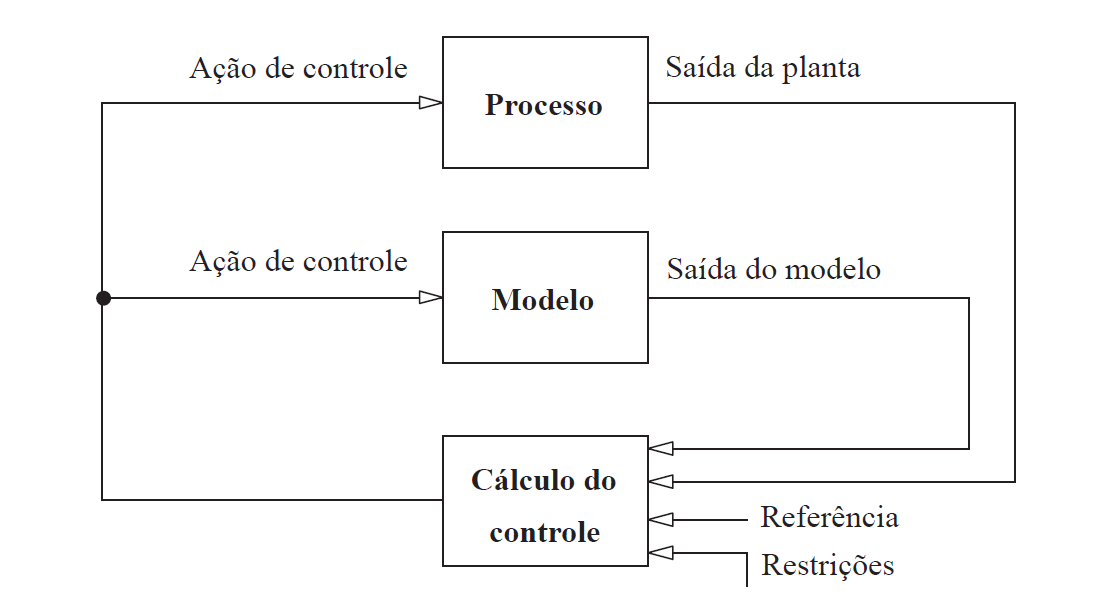
\includegraphics[scale=0.35]{figs/MPCbase.PNG} 
	   \caption{Algoritmo MPC}
	   \label{label para referencia cruzada Figura}
\end{figure}


% Lista de Item

\begin{itemize}
	\item item 1
	\item item 2
	\item item 3
\end{itemize}

% Equação
\begin{equation}
	\label{label para referencia cruzada equacoes} 
	y(t)=\sum_{i=1}^{\infty}h_i\Delta u(t-i)
\end{equation}

% Equação em linha 
$\hat{y}(t+k\mid t)= \sum^\infty_{i=1} g_i \Delta u(t+k-i\mid t)$

% Citação -  Criei o arquivo de bibliografia usando o jabref

\cite{Camacho2007} 

% Referencia Cruzada de Figura
\ref{label para referencia cruzada Figura}

% Referencia Cruzada de Equação
\ref{label para referencia cruzada equacoes}


% Tabelas

\begin{table}[h]
\begin{center}
     \caption{Índices 1 para casos factíveis}
     \begin{tabular}{| l | l | l | l |}
     \hline Índice & LP Petro & LP 2 & Diferença\\ 
     \hline $SES_y$& 60.5406 & 60.5492 & -0.0087\\
     \hline $SES_u$& 1166.1464 & 1166.1464 & 2.36*$10^{-9}$ \\
     \hline
     \end{tabular}
\label{table:indices1}
\end{center}
\end{table}
\chapter{Capítulos Subsequentes (2,3, etc)}

\textbf{Desenvolvimento:}(Fundamentação e Exposição do Assunto)

A partir do capítulo 1 começam os capítulos onde se: expõe, explica, demonstra, fundamenta, prova. É a comunicação dos trabalhos desenvolvidos e dos resultados obtidos. Geralmente isso dividido em vários capítulos, que devem começar com uma pequena introdução e terminar com uma conclusão, onde aspectos relevantes são convenientemente ressaltados.

No Capítulo 2, deve-se fazer uma descrição da empresa, processos, layouts, problemas, etc., ou seja, mais detalhadamente motivar e enquadrar o problema dentro do que proporão (a ser descrito no próximo capítulo).

\chapter{Conceitos Básicos}

\section{Métodos Ágeis de Desenvolvimento de Software}

\subsection{Agile}

\subsection{Scrum}

\section{Desenvolvimento de Aplicativos iOS}

\subsection{Sistema Operacional e Arquitetura da Plataforma}

\subsection{Ambiente de Desenvolvimento}

\subsection{Swift}

\subsection{Gerenciamento de Dependências}

\section{Versionamento de Código}

\section{RESTful API's}

\section{Testes Automatizados}
\missingfigure{Figuras classicas dos testes, modelo em V, piramide etc}
\subsection{Testes de UI}

\chapter{Gyymi}
Neste capítulo é apresentado o projeto do aplicativo Gyymi do ponto de vista do usuário do sistema. Os principais fluxos de uso do aplicativo são expostos, com comentários da parte técnico quando necessários.

% ********
% Cadastro
% ********
\section{Cadastro de Usuários e Estabelecimentos}
Ao entrar acessar o aplicativo pela primeira vez, o usuário encontra a tela de entrada (Figura \ref{fig:landing}). Nesta, três ações podem ser tomadas: cadastrar um estabelecimento (opção "I am a gym"), cadastrar um perfil de treinador (opção "I am a trainer") ou realizar o login na plataforma caso já tenha uma conta (opção "Login to existing account"). A seguir são detalhados os dois fluxos de cadastro do aplicativo.
\begin{figure}[H]
    \centering
    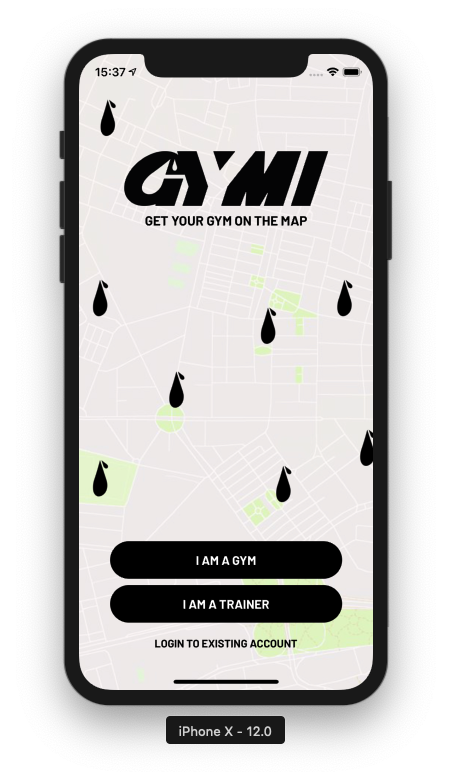
\includegraphics[width=0.4\textwidth]{pfc/figuras/landing.png}
    \caption{Tela de entrada do aplicativo}
    \label{fig:landing}
\end{figure}

% ******************
% Cadastro academias
% ******************
\subsection{Academias} \label{sec:register-gym}
Selecionada a opção por cadastro de um estabelecimento, o usuário primeiramente deve cadastrar os dados do administrador do local (ver Figura \ref{fig:register-manager-data}). Os seguintes dados são solicitados: primeiro nome, último nome, número do celular com código de área, e-mail (com campo de verificação) e senha (com campo de verificação). Para prosseguir com o cadastro, o usuário deve preencher os campos com dados válidos (caso contrário, alertas de erro são apresentados na tela). Ao clicar o botão "Next" uma chamada de API é feita ao back-end passando os dados digitados como parâmetro. Em caso de sucesso, a próxima tela do cadastro é apresentada; em caso de erro (como um e-mail de usuário já cadastrado), um alerta de erro é apresentado - Figura \ref{fig:register-manager-error}.

\begin{figure}[H]
	\centering
    \begin{subfigure}[b]{0.4\textwidth}
        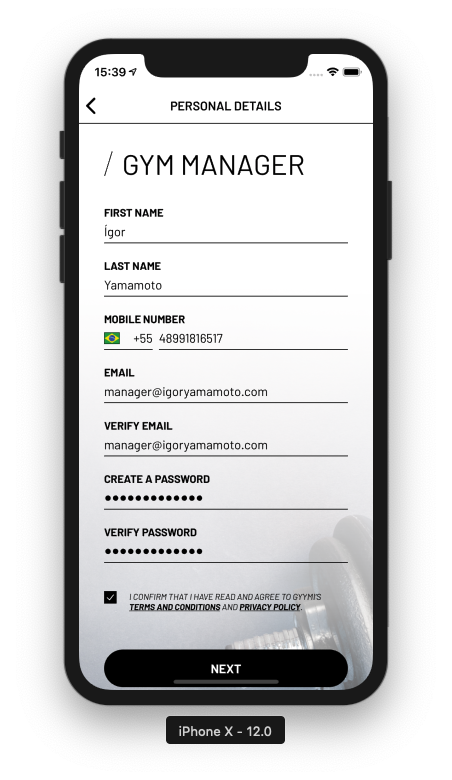
\includegraphics[width=\textwidth]{pfc/figuras/register-manager.png}
        \caption{Dados do administrador}
        \label{fig:register-manager-data}
    \end{subfigure}
    ~
	\begin{subfigure}[b]{0.4\textwidth}
        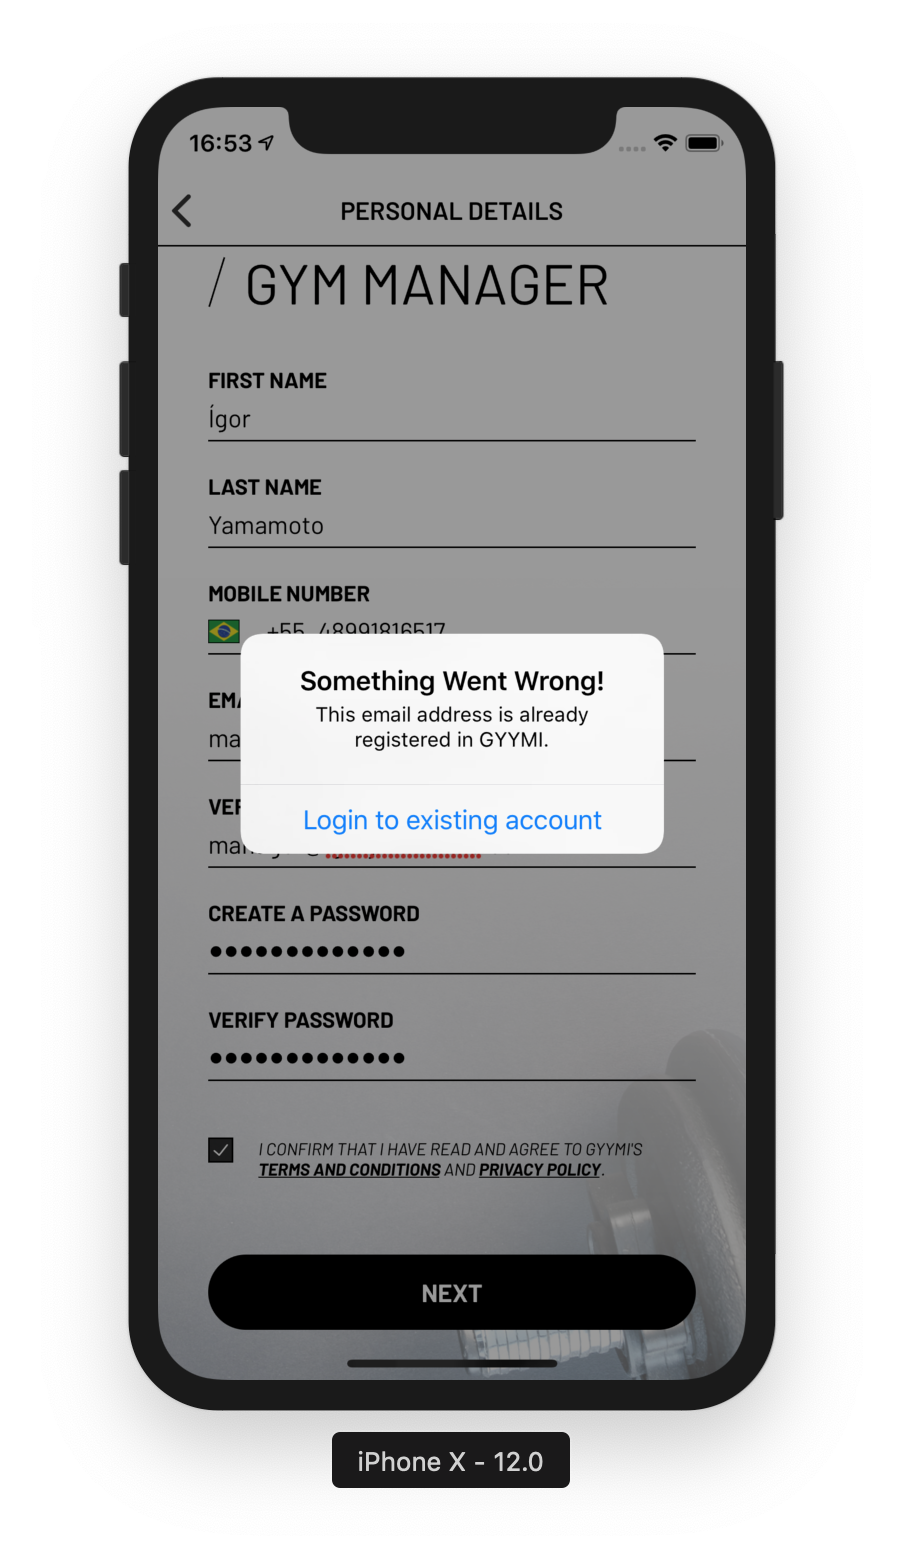
\includegraphics[width=\textwidth]{pfc/figuras/register-manager-error.png}
        \caption{Alerta de erro}
        \label{fig:register-manager-error}
    \end{subfigure}
    ~
    \caption{Tela de cadastro do usuário - administrador da academia}
    \label{fig:register-manager}
\end{figure}

Após o cadastro do usuário administrador da academia ter sido realizado com sucesso, o perfil do estabelecimento é cadastrado. Três telas fazem parte deste fluxo (ver Figura \ref{fig:register-gym}): primeiro informações gerais da academia (nome, endereço, número para contato com o estabelecimento, web-site e endereço de mídias sociais) devem ser passadas - Figura \ref{fig:register-gym-info}; em seguida um tela (Figura \ref{fig:register-gym-amenities}) com opções selecionáveis de facilidades e equipamentos fornecidos pela academia é apresentada; por último, o usuário tem a opção de carregar fotos do estabelecimento (Figura \ref{fig:register-gym-photos}), selecionando uma delas para ser exibida como foto de capa (a ser mostrada no perfil da academia).

\begin{figure}[H]
	\centering
    \begin{subfigure}[b]{0.3\textwidth}
        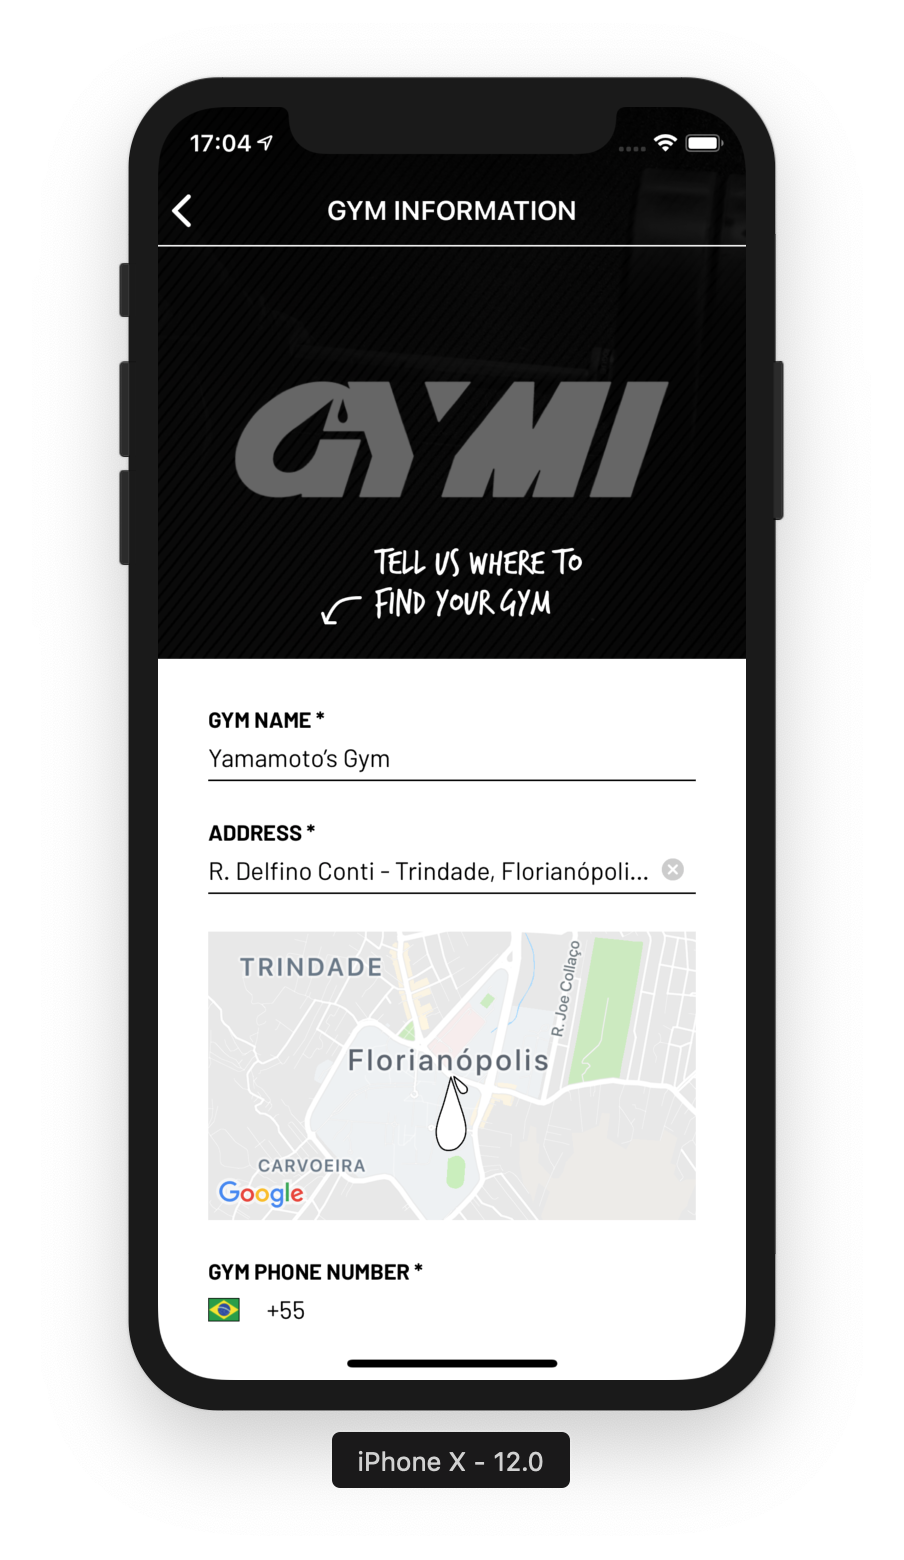
\includegraphics[width=\textwidth]{pfc/figuras/register-gym-info.png}
        \caption{Registro das informações gerais da academia}
        \label{fig:register-gym-info}
    \end{subfigure}
    ~
	\begin{subfigure}[b]{0.3\textwidth}
        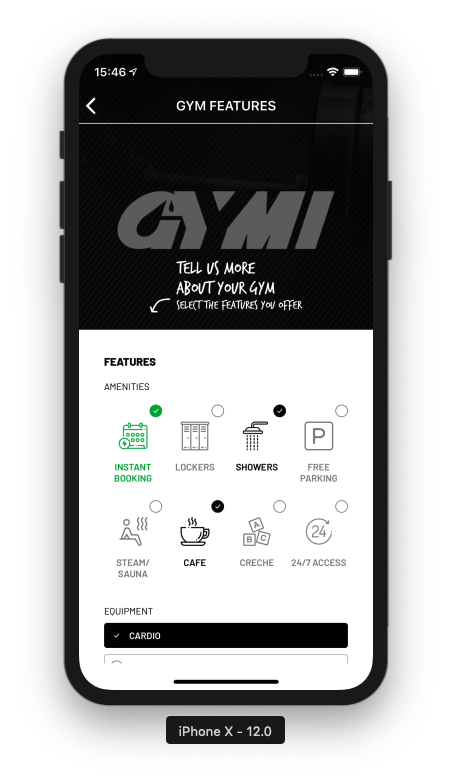
\includegraphics[width=\textwidth]{pfc/figuras/register-gym-amenities.png}
        \caption{Registro das facilidades e equipamentos}
        \label{fig:register-gym-amenities}
    \end{subfigure}
    ~
    \begin{subfigure}[b]{0.3\textwidth}
        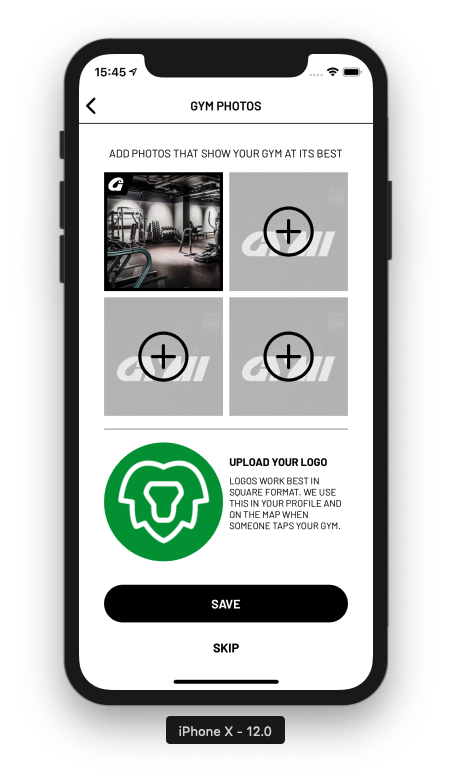
\includegraphics[width=\textwidth]{pfc/figuras/register-gym-photos.png}
        \caption{Registro das fotos do local e da logo}
        \label{fig:register-gym-photos}
    \end{subfigure}
    ~
    \caption{Telas de cadastro de um estabelecimento}
    \label{fig:register-gym}
\end{figure}

Ao término do cadastro do estabelecimento, uma tela de boas vindas (Figura \ref{fig:gym-welcome}) é apresentada ao usuário. A tela apresenta uma marcação (gota de suor branca) da academia em um mapa no local real cadastrado anteriormente (mapa obtido através do serviço do sistema de geolocalização, que é apresentado no próximo capítulo) e outros locais já cadastrados na plataforma são demarcados também (gotas pretas de suor menores), informação proveniente do back-end. A tela apresenta duas opções de ação: registrar detalhes da conta bancária (opção "Add bank details", tela não implementada para a versão piloto do aplicativo) e uma opção para pular o cadastro da conta (opção "Skip"). Ambas as ações levam o usuário as telas de uso da academia, que são apresentadas nas próximas secções.

\begin{figure}[ht]
    \centering
    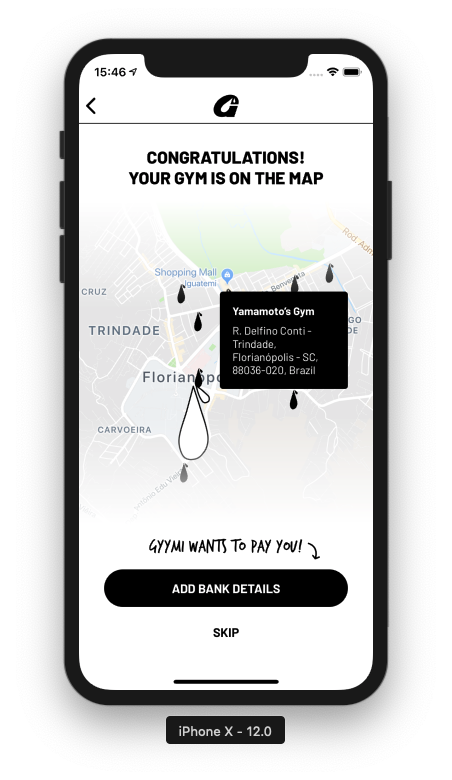
\includegraphics[width=0.4\textwidth]{pfc/figuras/gym-welcome.png}
    \caption{Tela de boas vindas para o estabelecimento}
    \label{fig:gym-welcome}
\end{figure}

% ********************
% Cadastro Treinadores
% ********************
\subsection{Treinadores}
Caso o usuário selecione a opção de cadastro de um treinador na tela de entrada, o mesmo é redirecionado para a tela de cadastro de informações gerais de usuário (Figura \ref{fig:register-trainer-info}), com os seguintes campos de dados: primeiro nome, último nome, e-mail, número do celular, senha (com campo de verificação). Caso as informações preenchidas sejam válidas, o cadastro prossegue para a próxima tela; caso contrário, alertas de erros são exibidos (como no caso do estabelecimento - Secção \ref{sec:register-gym})

Após o preenchimento dos campos, uma requisição para registrar os dados na plataforma é feita para o back-end, o qual faz uma requisição ao serviço de envio de SMS com os dados do número do celular do usuário. Este serviço então envia um SMS com um código de verificação, que deve ser preenchido no campo "Verification Code" da tela de verificação por SMS (ver Figura \ref{fig:register-trainer-verification}). Nesta tela o usuário tem duas opções de ação: verificar o código preenchido (opção que dispara uma nova requisição ao back-end para identificar se o código fornecido é o mesmo gerado pelo serviço de SMS) ou reenviar o código de verificação (opção que desencadeia um novo envio de SMS para o usuário através de nova solicitação para tal ao serviço de SMS).

\begin{figure}[H]
	\centering
    \begin{subfigure}[b]{0.4\textwidth}
        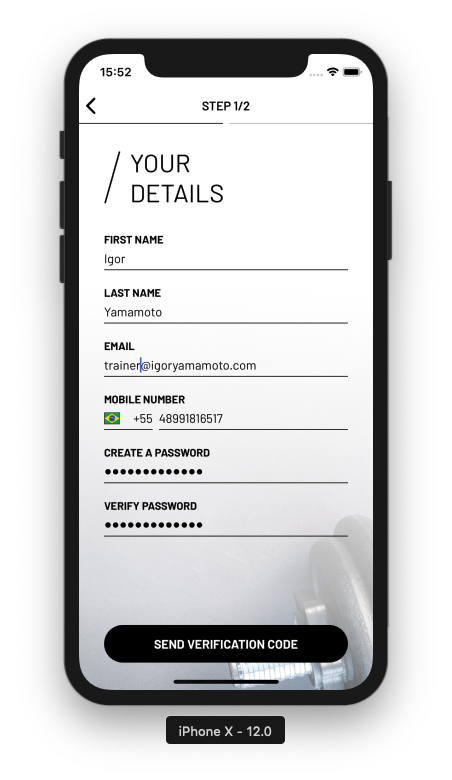
\includegraphics[width=\textwidth]{pfc/figuras/register-trainer.png}
        \caption{Dados do treinador}
        \label{fig:register-trainer-info}
    \end{subfigure}
    ~
	\begin{subfigure}[b]{0.4\textwidth}
        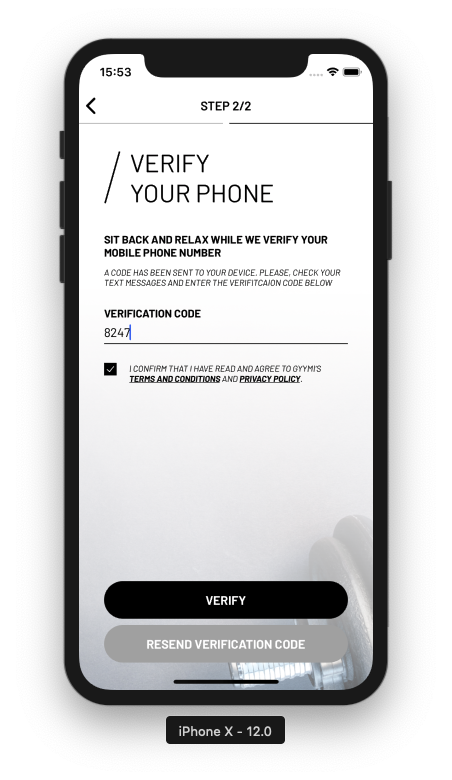
\includegraphics[width=\textwidth]{pfc/figuras/register-trainer-verification.png}
        \caption{Verificação por SMS}
        \label{fig:register-trainer-verification}
    \end{subfigure}
    ~
    \caption{Tela de cadastro do usuário - treinador pessoal}
    \label{fig:register-trainer}
\end{figure}

Uma vez que o código de verificação é validado, o fluxo prossegue para uma tela de boas vindas (Figura \ref{fig:tr-welcome}). Nesta tela, o usuário tem a ação de configurar seu perfil de treinador (opção "Set up your trainer profile") ou a ação de pular esta etapa (opção "Skip"). Caso selecionada a opção de configuração, o cadastro prossegue; caso selecionada a outra opção, o usuário é direcionado a tela principal do treinador.

\begin{figure}[H]
    \centering
    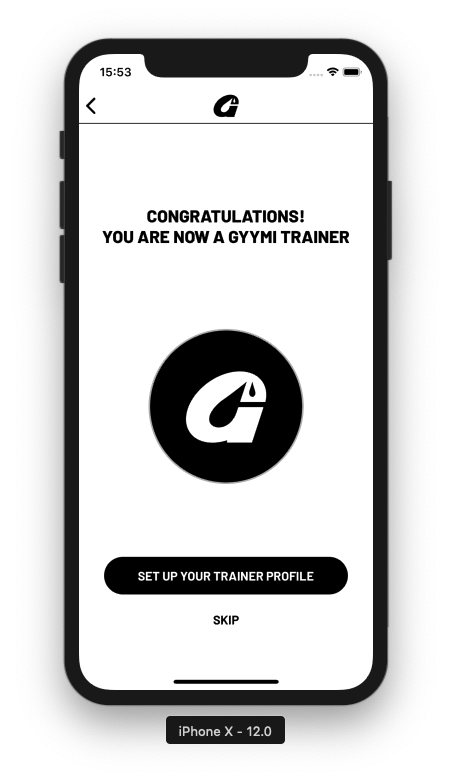
\includegraphics[width=0.4\textwidth]{pfc/figuras/tr-congratulations.png}
    \caption{Tela de boas vindas para o treinador}
    \label{fig:tr-welcome}
\end{figure}

A configuração de perfil de treinador segue um fluxo de três telas (Figura \ref{fig:register-tr-profile}). Primeiro, o usuário deve registrar as informações gerais do perfil (Figura \ref{fig:register-tr-profile-info}), informando de forma opcional os campos: mantra, área de treino, endereço de mídias sociais e web-site. Em seguida, o usuário é direcionado a uma tela com opções selecionáveis de habilidades e especialidades (Figura \ref{fig:register-tr-skills}) que ele pode oferecer em seus treinos físicos. Por último, uma tela de confirmação do cadastro do perfil é exibida (Figura \ref{fig:register-tr-profile-confirmation}), com opções de edição caso o usuário deseje alterar alguma informação. Ao pressionar o botão de confirmar, uma requisição é feita ao back-end passando os dados de perfil do treinador para registro no sistema. Após a requisição ter obtido sucesso, o usuário é direcionado a tela principal de uso do aplicativo do treinador, a ser apresentada nas próximas secções.

\begin{figure}[H]
	\centering
    \begin{subfigure}[b]{0.3\textwidth}
        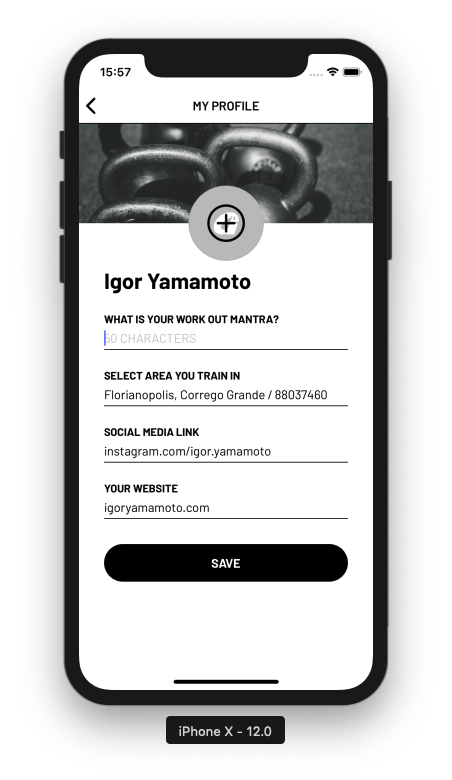
\includegraphics[width=\textwidth]{pfc/figuras/tr-register-profile-1.png}
        \caption{Registro das informações gerais do treinador}
        \label{fig:register-tr-profile-info}
    \end{subfigure}
    ~
	\begin{subfigure}[b]{0.3\textwidth}
        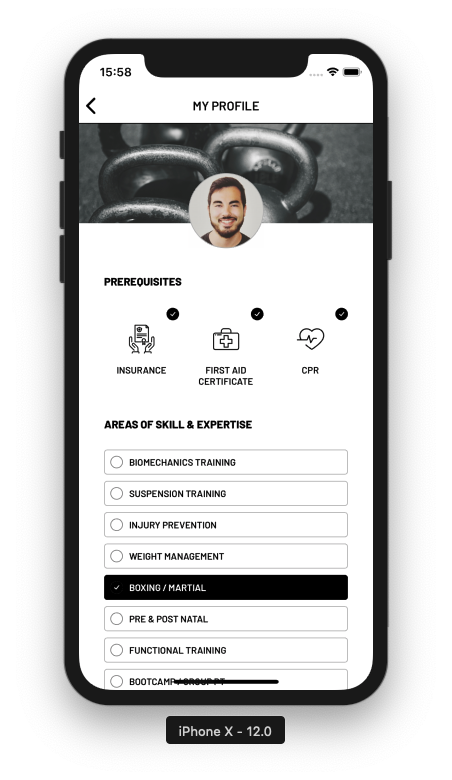
\includegraphics[width=\textwidth]{pfc/figuras/tr-register-profile-2.png}
        \caption{Registro das habilidades e especialidades}
        \label{fig:register-tr-skills}
    \end{subfigure}
    ~
    \begin{subfigure}[b]{0.3\textwidth}
        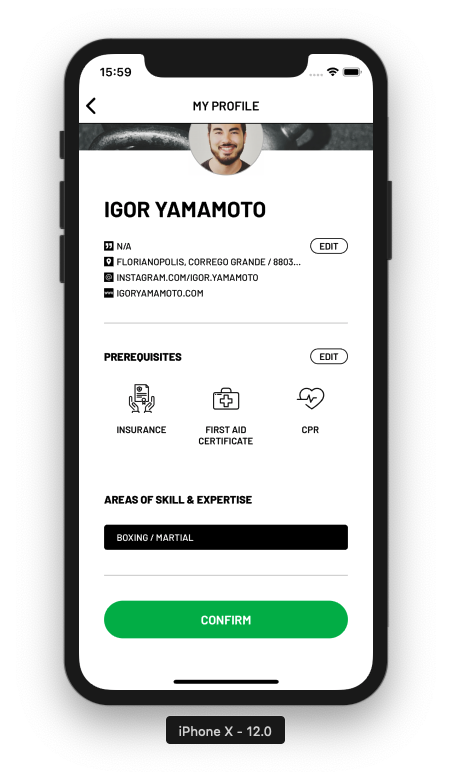
\includegraphics[width=\textwidth]{pfc/figuras/tr-register-profile-3.png}
        \caption{Confirmação do registro de perfil}
        \label{fig:register-tr-profile-confirmation}
    \end{subfigure}
    ~
    \caption{Fluxo de cadastro de perfil de treinador}
    \label{fig:register-tr-profile}
\end{figure}

% *******************
% Interface academias
% *******************
\section{Interface para Academias}
Nesta secção, é apresentada a interface de uso dos usuários que cadastraram um estabelecimento na plataforma. As principais funcionalidades implementadas para a versão piloto do aplicativo são abordadas: dashboard com dados semanais de uso da academia, calendário de sessões agendadas e configuração de agenda semanal para locação, perfil da academia.

Na interface para as academias o usuário tem a opção de navegar por cinco telas principais, selecionadas a partir da barra de navegação na parte inferior do aplicativo (Figura \ref{fig:gym-tabbar}). Da esquerda para a direita, as opções de navegação são: dashboard da academia; treinadores com sessões agendadas (não implementado para o piloto); calendário de sessões agendadas; central de notificações (não implementado para o piloto); perfil do estabelecimento.

Todos os dados que aparecem nas telas são provenientes de chamadas de API feitas ao back-end da aplicação. De acordo com o endpoint acessado, o back-end realiza o acesso ao banco de dados remoto da aplicação, efetua cálculos e aplica as lógicas de negócio se necessário. Em seguida, o mesmo envia a resposta à requisição. A chamada geralmente é feita no momento em que os componentes da tela são carregados ou imediatamente antes de serem renderizados. Mais detalhes desta integração são discutidos no próximo capítulo.

\begin{figure}[H]
    \centering
    
\includegraphics{pfc/figuras/gym-tabbar.png}
    \caption{Barra de navegação da interface para academias}
    \label{fig:gym-tabbar}
\end{figure}


\subsection{Dashboard da Academia}
A tela de dashboard da academia (Figura \ref{fig:gym-dashboard}) apresenta dados de uso e de receita semanais do estabelecimento. Os seguintes dados da semana corrente e anterior são apresentados no painel: receita total, número total de agendamentos, número total de treinadores, número total de hora agendadas por treinadores.

\begin{figure}[H]
    \centering
    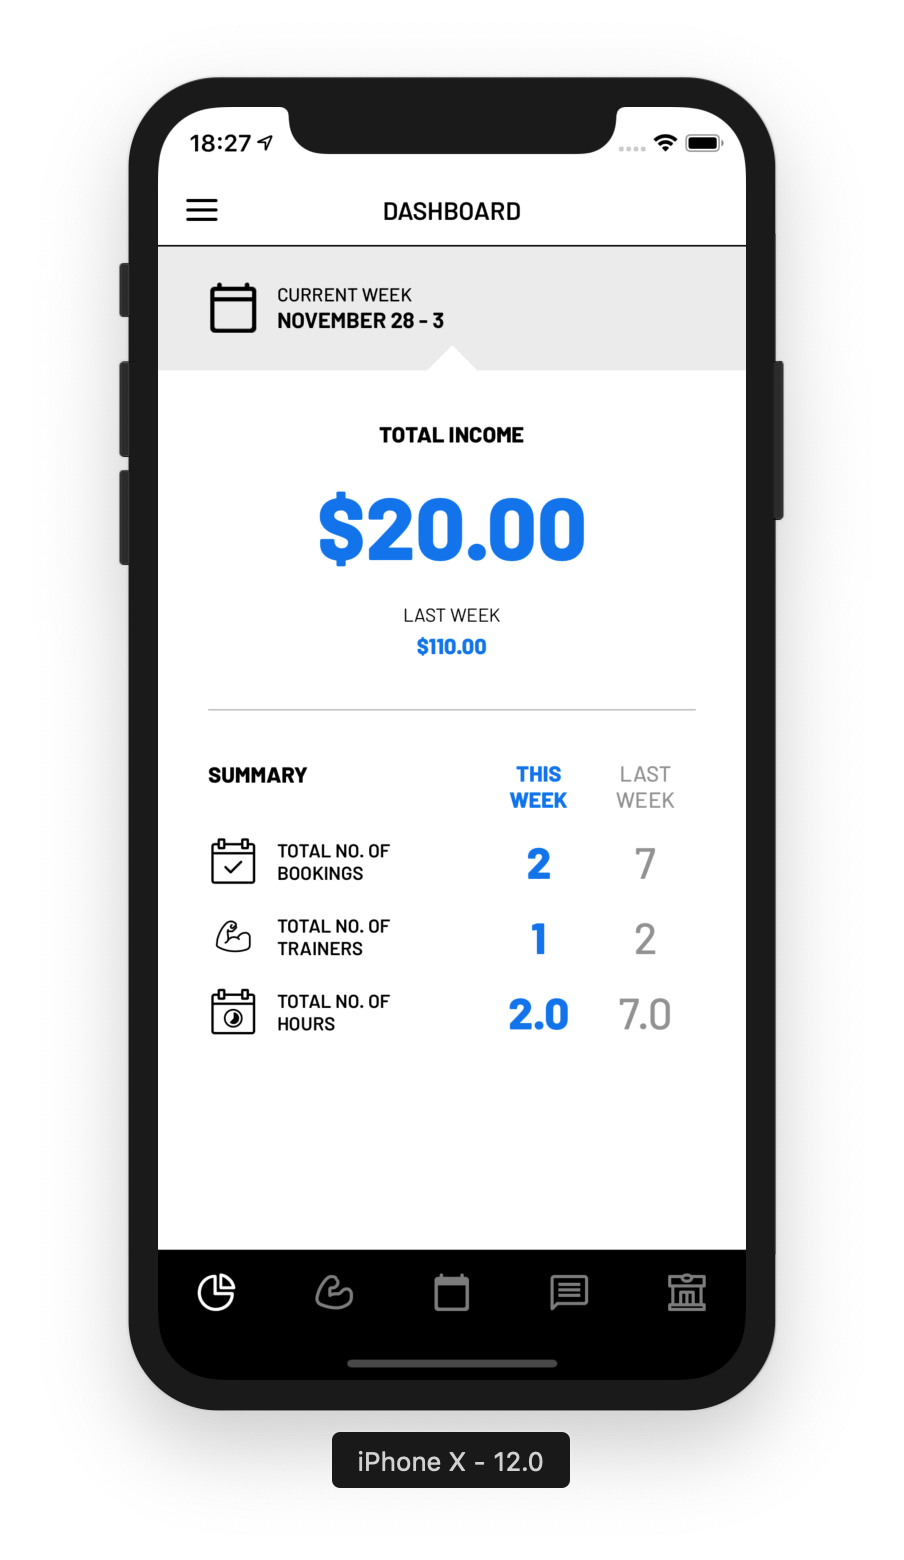
\includegraphics[width=0.4\textwidth]{pfc/figuras/gym-dashboard.png}
    \caption{Tela de dashboard da academia}
    \label{fig:gym-dashboard}
\end{figure}

\subsection{Agenda Semanal para Locação}
Ao acessar pela primeira vez a interface das academias, o usuário é direcionado para uma tela (ver Figura \ref{fig:gym-block-onboard}) onde são passadas informações de como funciona a agenda de blocos de horários semanais para locação da academia. A aplicação permite que as academias cadastrem blocos de horários fixos para cada dia da semana. Cada bloco contém a informação de taxa cobrada por hora, máximo número de pessoas permitidas e limites inferior e superior de horário para sessões. A partir destes blocos, os treinadores podem agendar sessões dentro dos mesmos (selecionando o número de clientes que eles vão levar, respeitando o limite máximo, e escolhendo o horário de início e término de uma sessão dentro dos limites de horário do bloco).

A Figura \ref{fig:gym-add-block} ilustra a tela de adição de um bloco semanal. As seguintes informações devem ser passadas: horários limites de início e término das sessões de treino, seleção de dias da semana nos quais o bloco será aplicado (ou seja, se academia quer disponibilizar blocos idênticos para diferentes dias da semana, ela utiliza esta opção), máximo número de pessoas permitidas dentro do bloco em um dado momento e, por último, taxa por hora cobrada dos treinadores.

Após a adição de blocos, os mesmos são exibidos na agenda (Figura \ref{fig:gym-block}) na posição correspondente aos limites de horário do bloco (blocos não podem ter limites de horários sobrepostos). Ao clicar no botão "Edit", o usuário pode editar as informações do bloco previamente fornecidas.

\begin{figure}[H]
	\centering
    \begin{subfigure}[b]{0.3\textwidth}
        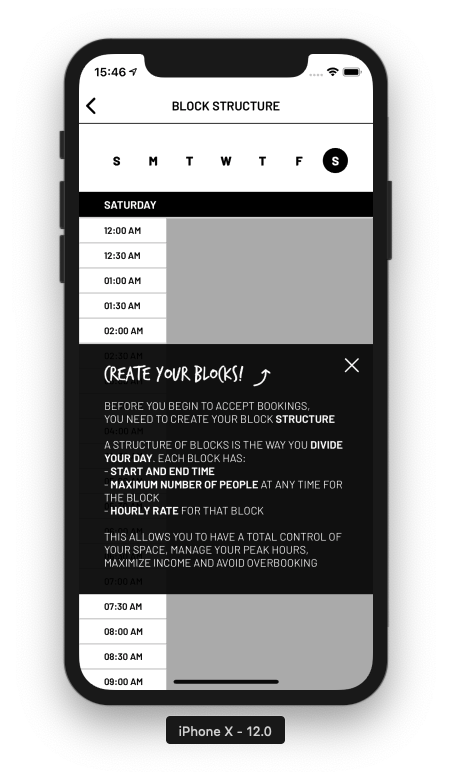
\includegraphics[width=\textwidth]{pfc/figuras/gym-block-structure-onboard.png}
        \caption{Instruções da agenda semanal}
        \label{fig:gym-block-onboard}
    \end{subfigure}
    ~
	\begin{subfigure}[b]{0.3\textwidth}
        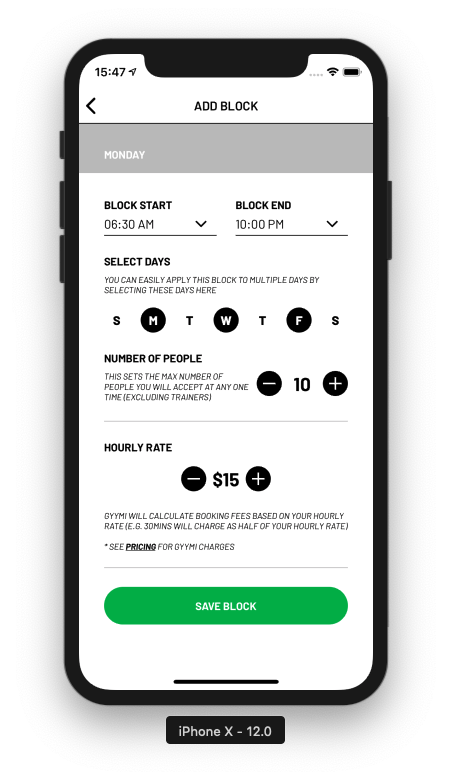
\includegraphics[width=\textwidth]{pfc/figuras/gym-add-block.png}
        \caption{Adição de novo bloco semanal}
        \label{fig:gym-add-block}
    \end{subfigure}
    ~
    \begin{subfigure}[b]{0.3\textwidth}
        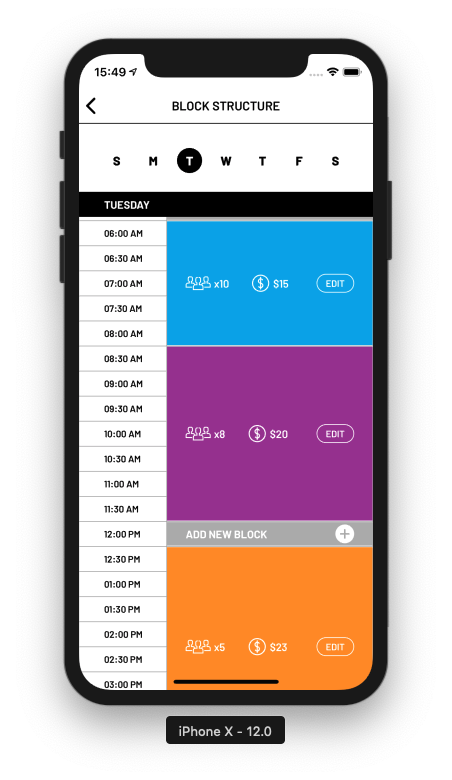
\includegraphics[width=\textwidth]{pfc/figuras/gym-block-structure.png}
        \caption{Agenda semanal da academia populada}
        \label{fig:gym-block}
    \end{subfigure}
    ~
    \caption{Fluxo de criação de blocos de horários para agenda semanal das academias}
    \label{fig:}
\end{figure}

\subsection{Calendário de Sessões Agendadas}
A tela de calendário de sessões agendadas (Figura \ref{fig:gym-calendar}) mostra informações gerais de agendamento de sessões filtradas por data. Na parte superior da interface, é possível selecionar a data em que se deseja obter informações através de um calendário. Em seguida dados da data selecionada são exibidos (número de treinadores e clientes do dia e receita esperada para o dia). Por fim, uma agenda com os blocos do dia é apresentada, com a indicação de quantos treinadores e seus respectivos clientes marcaram sessões de treino em cada bloco.

Ao clicar o botão "View details" localizado em cada um dos blocos, a tela de detalhes de agendamentos (Figura \ref{fig:gym-booking-detail}) é exibida. Nesta tela, todas as sessões agendadas no bloco selecionado são listadas. Cada sessão é detalhada em um card, contendo o nome completo do treinador, horários de início e término da sessão, total a pagar e número de clientes que o mesmo vai levar ao estabelecimento.

\begin{figure}[H]
	\centering
    \begin{subfigure}[b]{0.4\textwidth}
        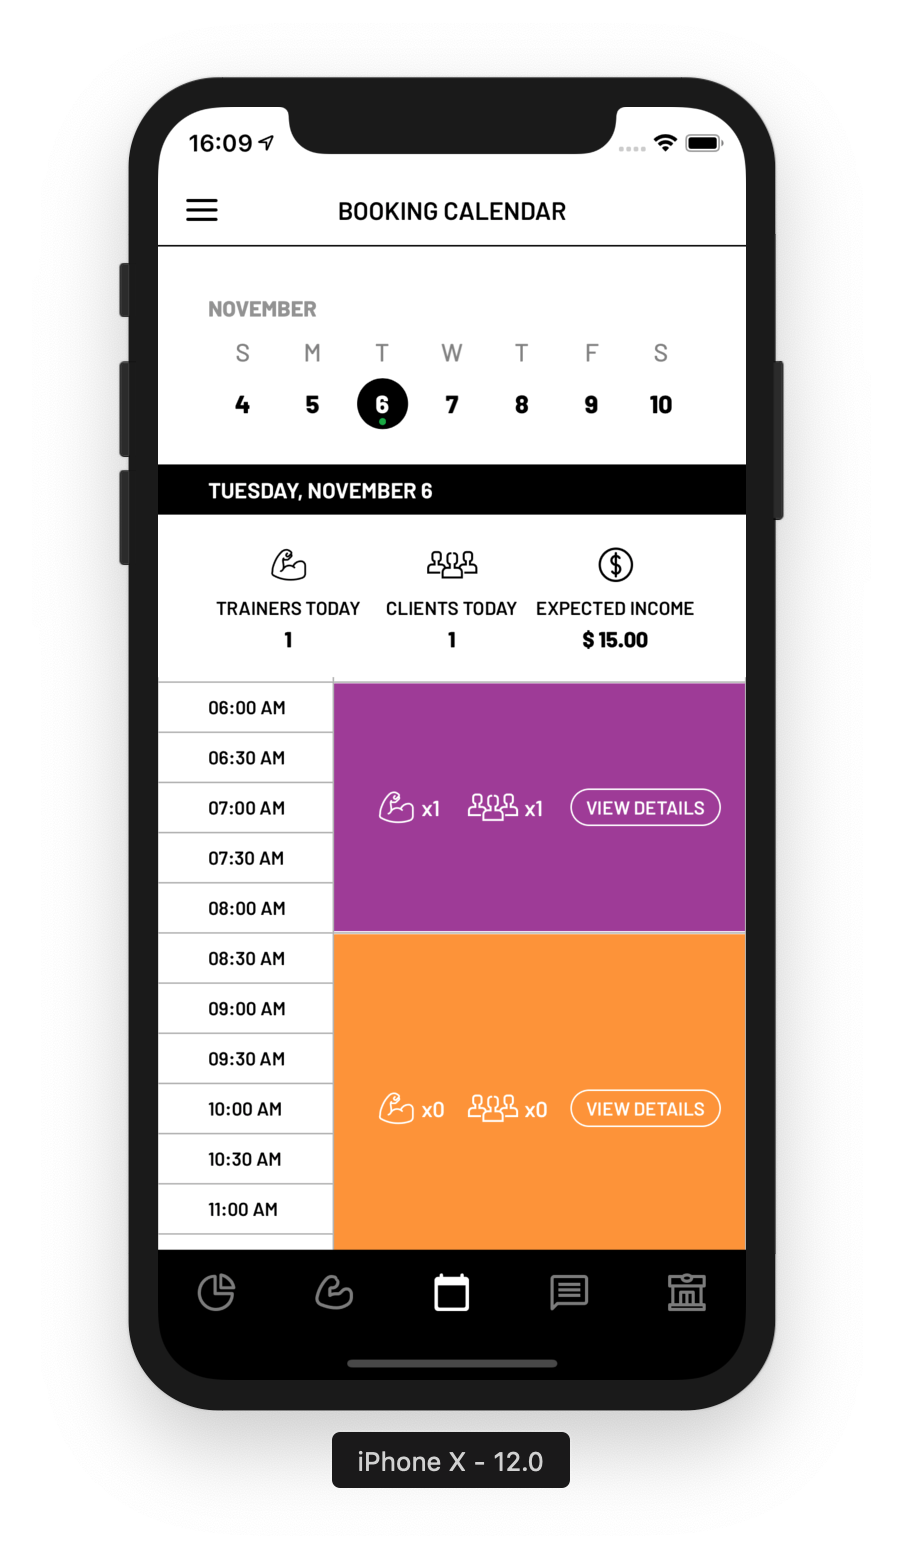
\includegraphics[width=\textwidth]{pfc/figuras/gym-booking-calendar.png}
        \caption{Calendário de sessões}
        \label{fig:gym-booking-calendar}
    \end{subfigure}
    ~
	\begin{subfigure}[b]{0.4\textwidth}
        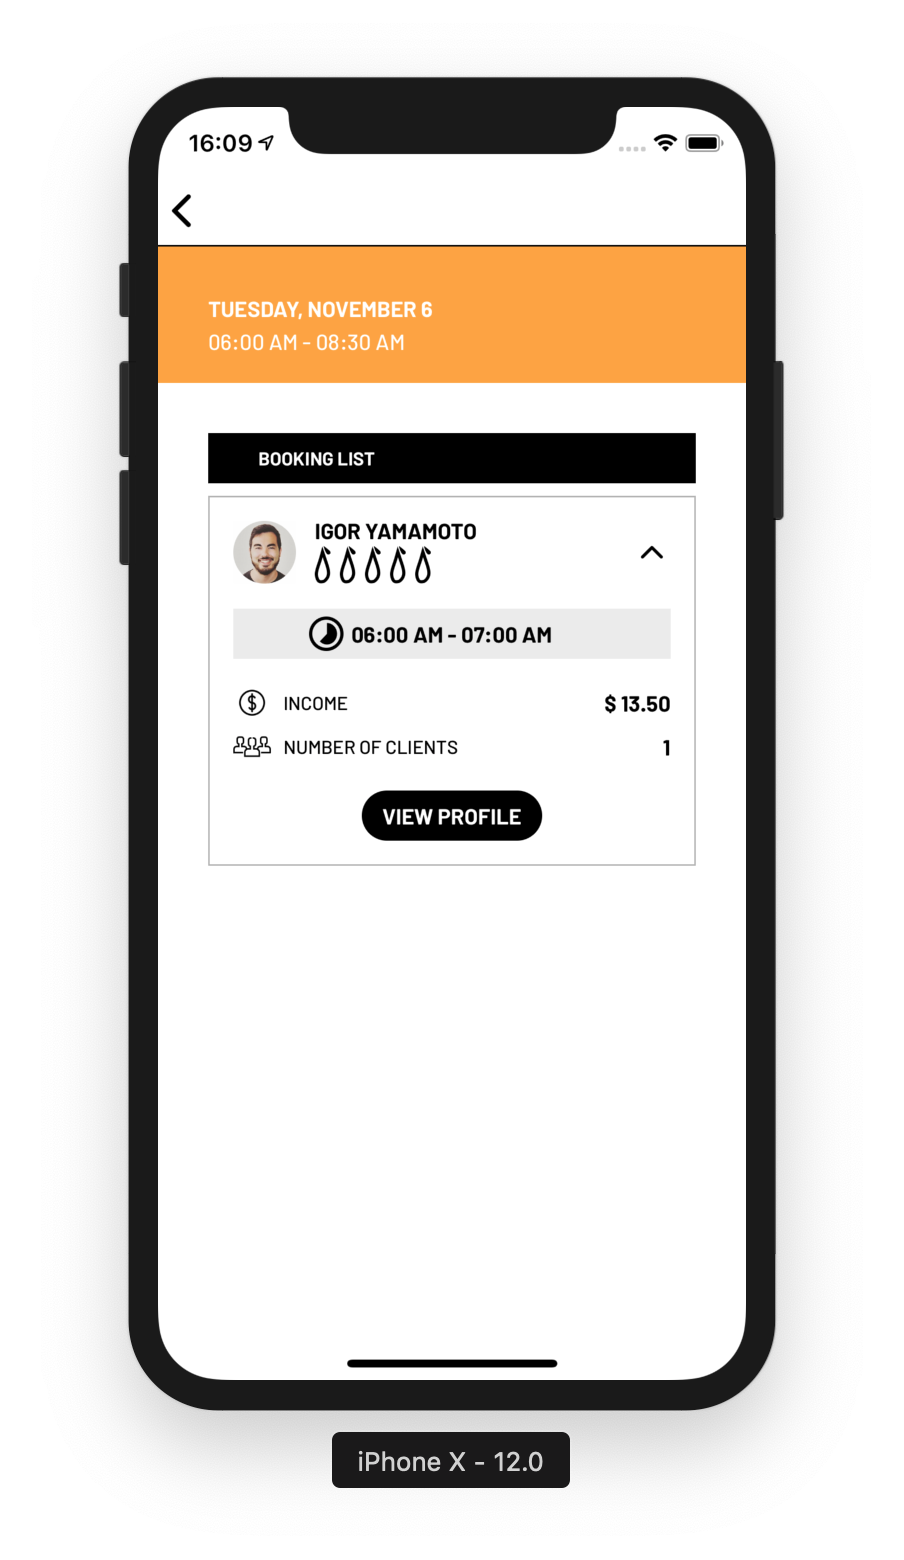
\includegraphics[width=\textwidth]{pfc/figuras/gym-booking-detail.png}
        \caption{Detalhes da sessão}
        \label{fig:gym-booking-detail}
    \end{subfigure}
    ~
    \caption{Telas do calendário de sessões agendadas na academia}
    \label{fig:gym-calendar}
\end{figure}

\subsection{Perfil do Estabelecimento}
A tela de perfil da academia além de exibir todos os dados passados pelo usuário no momento do cadastro, também mostra um indicador da nota do estabelecimento (de $1$ a $5$, calculada como sendo a média das avaliações de sessões de treino) e um mapa com a marcação da localização da academia. A interface permite que o usuário clique no botão "Edit" para que possa realizar edições no perfil previamente preenchido no momento do cadastro.

\begin{figure}[H]
    \centering
    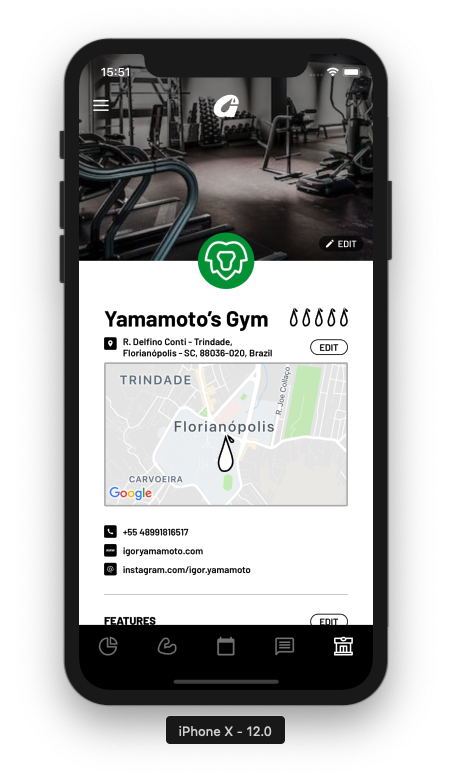
\includegraphics[width=0.4\textwidth]{pfc/figuras/gym-profile.png}
    \caption{Tela de perfil da academia}
    \label{fig:gym-profile}
\end{figure}

% *********************
% Interface treinadores
% *********************
\section{Interface para Treinadores}



\subsection{Busca por Academias}

\subsection{Agendamento de Sessão}

\subsection{Calendário de Sessões Agendadas}

\subsection{Perfil do Treinador}
\chapter{Implementação e Integração do Aplicativo} \label{cap:development}
Neste capítulo são apresentadas as implementações e integrações de sistemas realizadas para o aplicativo iOS. Somente as partes do projeto em que o autor esteve envolvido são apresentadas. Portanto, os detalhes de implementação do aplicativo para o sistema Android e do back-end da aplicação não são abordados, assim como a elaboração do design gráfico das telas. O autor teve participação central nas implementações do aplicativo iOS e integração de sistemas.

\section{Arquitetura da Aplicação}
A arquitetura global da aplicação é ilustrada na Figura \ref{fig:architecture}. O diagrama tem os principais sistemas de software representados pelas caixas e a comunicação entre os mesmos representada pelas setas. 

O banco de dados é isolado em ambiente remoto, através do serviço da empresa Amazon, e é acessado diretamente apenas pelo back-end. Este é responsável por implementar a maior parte da lógica de negócio da aplicação, fornecendo respostas às requisições feitas pelo aplicativo iOS. O back-end se comunica com o serviço de envio de SMS para requisitar e validar códigos de verificação. Também se comunica com o serviço de pagamento para emitir pedidos de transação. O aplicativo iOS consiste no sistema que define como todas as interações com o usuário final ocorrem, além de ser o responsável por apresentar visualmente todo o conteúdo da aplicação. O aplicativo iOS se comunica com o serviço de geolocalização para a apresentação de mapas e se comunica com o serviço de pagamento para enviar dados de pagamento do usuário final, como números de cartão de crédito.

\begin{figure}[H]
    \centering
    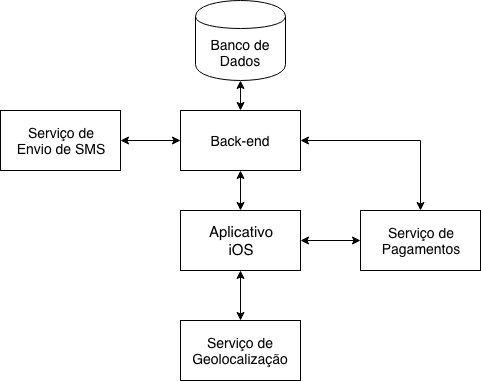
\includegraphics[width=0.8\textwidth]{pfc/figuras/system-architecture.png}
    \caption{Arquitetura global dos sistemas envolvidos}
    \label{fig:architecture}
\end{figure}


\section{Banco de Dados}
O banco de dados da aplicação está localizado na nuvem, através do serviço de acesso remoto da Amazon. O banco de dados projetado segue o modelo relacional, o qual foi julgado suficiente para representar os dados armazenados na aplicação e por ser extensamente utilizado em aplicações similares (que requerem cadastro e armazenamento de dados de usuários e outras entidades).

A Figura \ref{fig:database} ilustra o modelo de dados projetado através do diagrama de entidades. O modelo de dados está centrado nas entidades de usuário ("User"), academia ("Gym") e agendamento ("Booking") de forma a captar a principal funcionalidade da aplicação que é conectar treinadores (usuários) e academias através de agendamentos de treinos.

\begin{figure}[H]
    \centering
    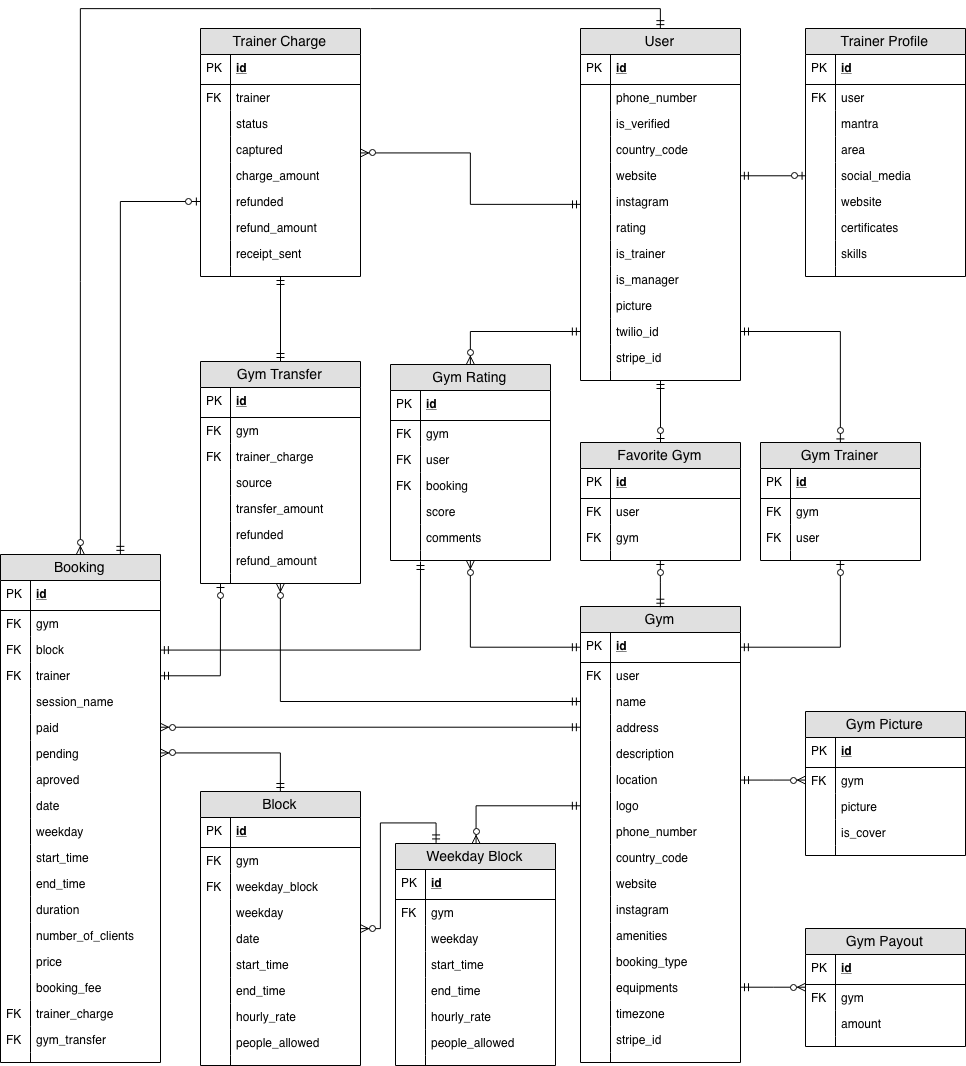
\includegraphics[width=0.8\textwidth]{pfc/figuras/database-schema.png}
    \caption{Diagrama do modelo de dados relacional}
    \label{fig:database}
\end{figure}

\section{Aplicativo iOS}
Nesta seção são apresentados os detalhes de cada camada da arquitetura do aplicativo iOS, com exemplos de implementação. Em seguida, são apresentados os critérios de avaliação das implementações. Por fim, são apresentados os desafios e dificuldades da implementação do aplicativo iOS.

% *******
% Modelos
% *******
\subsection{\textit{Model}: Representação de Dados}
Os dados da aplicação são representados localmente no aplicativo iOS através de \textit{struct}'s, estrutura de dado da linguagem Swift. Uma \textit{struct} no Swift permite definir propriedades e armazenar valores, definir métodos e inicializadores, além de permitir a conformação com protocolos. Os dados apresentados no aplicativos são provenientes dos retornos das chamadas de API's e são armazenados, em sua maioria, de forma volátil no aplicativo, na memória do dispositivo. Apenas alguns dados são persistidos no dispositivo: os dados do modelo de usuário e academia são mantidos para acesso rápido; o \textit{token} de autenticação do usuário também é mantido no dispositivo para que o mesmo possa manter sua sessão atual ativa, mesmo após fechar o aplicativo.


A Figura \ref{fig:user-model} exemplifica a representação de dados no aplicativo através do modelo de usuário. A \textit{struct} contém as propriedades relacionadas ao usuário, com os respectivos tipos de dados associados. O protocolo \textit{Codable} é utilizado para permitir a tradução automática de dados da API, convertendo-os em uma instância da \textit{struct}. O modelo de usuário contém ainda uma variável computada ("fullName"), ou seja, calculada a partir de propriedades armazenadas.

\begin{figure}[H]
    \centering
    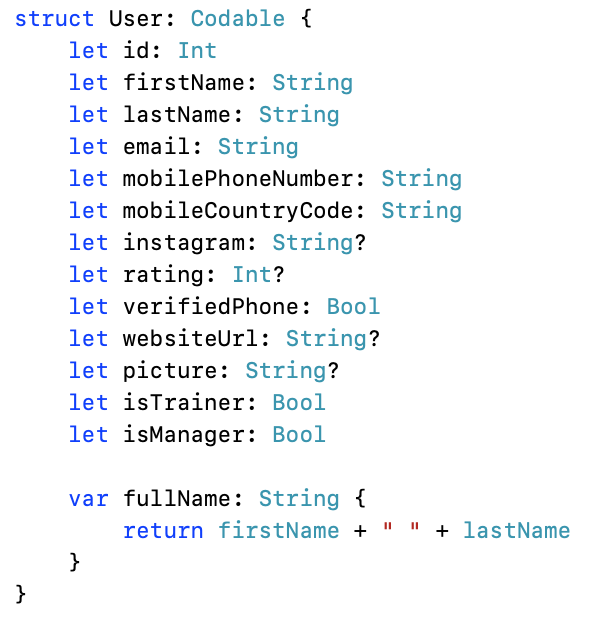
\includegraphics[width=0.6\textwidth]{pfc/figuras/user-model.png}
    \caption{Exemplo de modelo local de dados no aplicativo iOS}
    \label{fig:user-model}
\end{figure}

% **********
% Controller
% **********
\subsection{\textit{Controller}: Lógica e Tratamento de Ações}
A camada que controla a parte lógica do aplicativo e o tratamento de ações (em resposta à interações com o usuário) foi implementada com \textit{UIViewControllers}, classe base para controladores fornecida pelo framework UIKit. Os controladores foram separados em classes que tratam, em linhas gerais, da lógica de uma tela específica do aplicativo. Assim, os mesmos são responsáveis por definir o comportamento das telas em cada etapa de seu ciclo de vida, além de responder às interações associadas a elementos da interface em questão. Também realizam a chamada de métodos da camada de redes do aplicativo, em que chamadas de API's são feitas, e atualizam a interface gráfica com os dados recebidos.

A Figura \ref{fig:controller-example} contém um trecho de código de um exemplo de controlador. O exemplo implementa o controlador responsável pela lógica do dashboard de treinadores. No trecho de código é possível visualizar a propriedade "dashboard", que quando sobrescrita, chama um método para atualizar os dados da interface gráfica ("setupDashboardData()"). Também é possível ver o controle do comportamento da tela nas etapas de ciclo de vida em que: teve seus elementos de interface carregados ("viewDidLoad()") e está prestes a ser renderizada ("viewWillAppear()"). Nestas etapas, são chamados diversos métodos que controlam o comportamento da tela, como configuração de aspectos de aparência ("setupView()"), atualização de textos de acordo com a localização do dispositivo ("setupLocalizables()"), entre outros.

\begin{figure}[H]
    \centering
    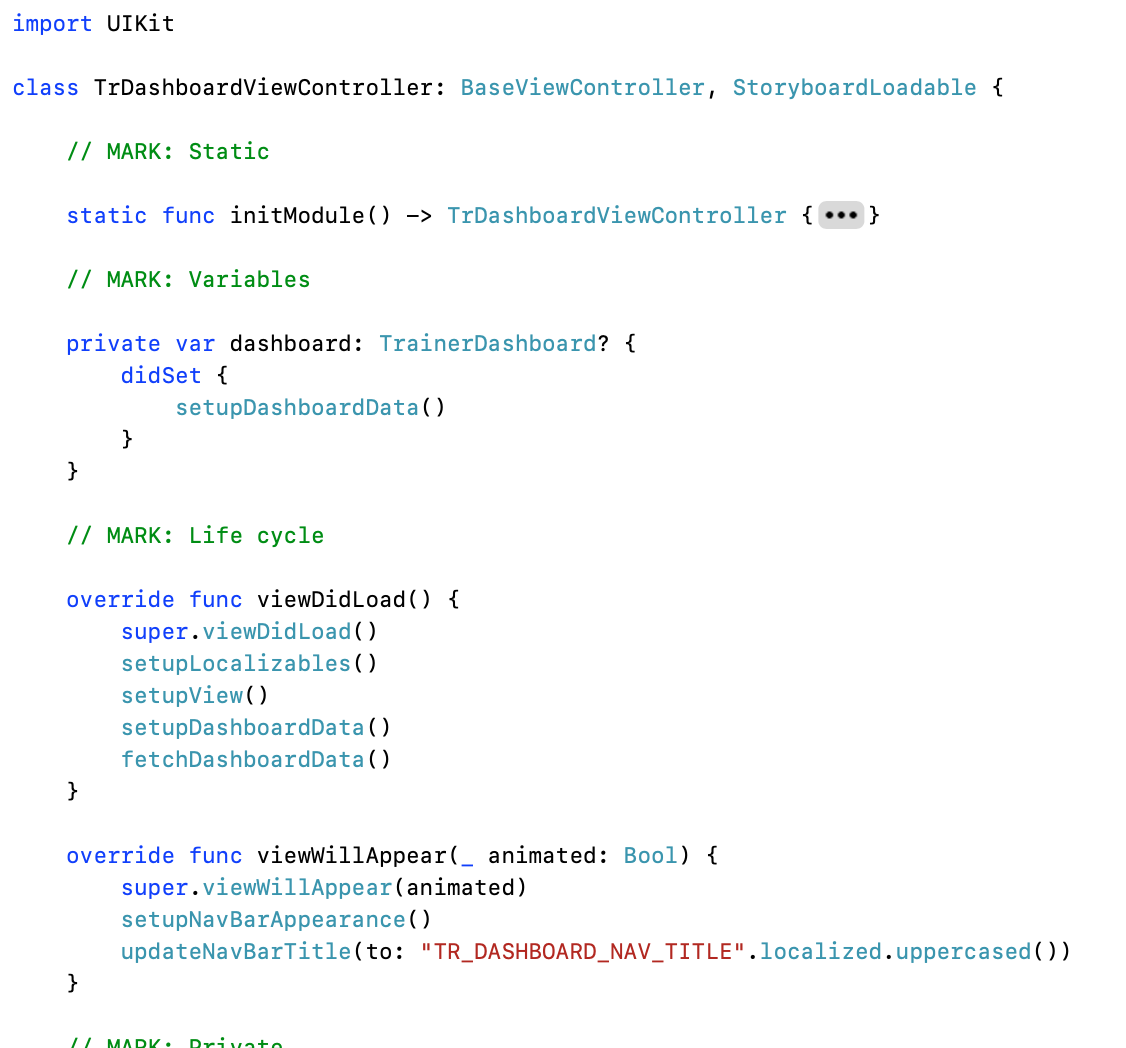
\includegraphics[width=0.9\textwidth]{pfc/figuras/ex-tr-dashboard.png}
    \caption{Exemplo de implementação de controladores no aplicativo iOS}
    \label{fig:controller-example}
\end{figure}

% *****************
% Interface Gráfica
% *****************
\subsection{\textit{View}: Interface Gráfica}
A implementação das interfaces gráficas do aplicativo foi feita principalmente com o uso de \textit{Storyboard}'s, ferramenta gráfica de construção de interfaces do Xcode. A Figura \ref{fig:storyboard} ilustra o uso de um \textit{Storyboard} para a construção da tela de entrada do aplicativo. Na parte esquerda da figura, é apresentada a hierarquia dos componentes da interface. Na região central, os elementos são dispostos na tela de acordo com o dispositivo selecionado. Na direita, encontram-se especificações de restrições de layout impostas ao componente da interface selecionado.

\begin{figure}[H]
    \centering
    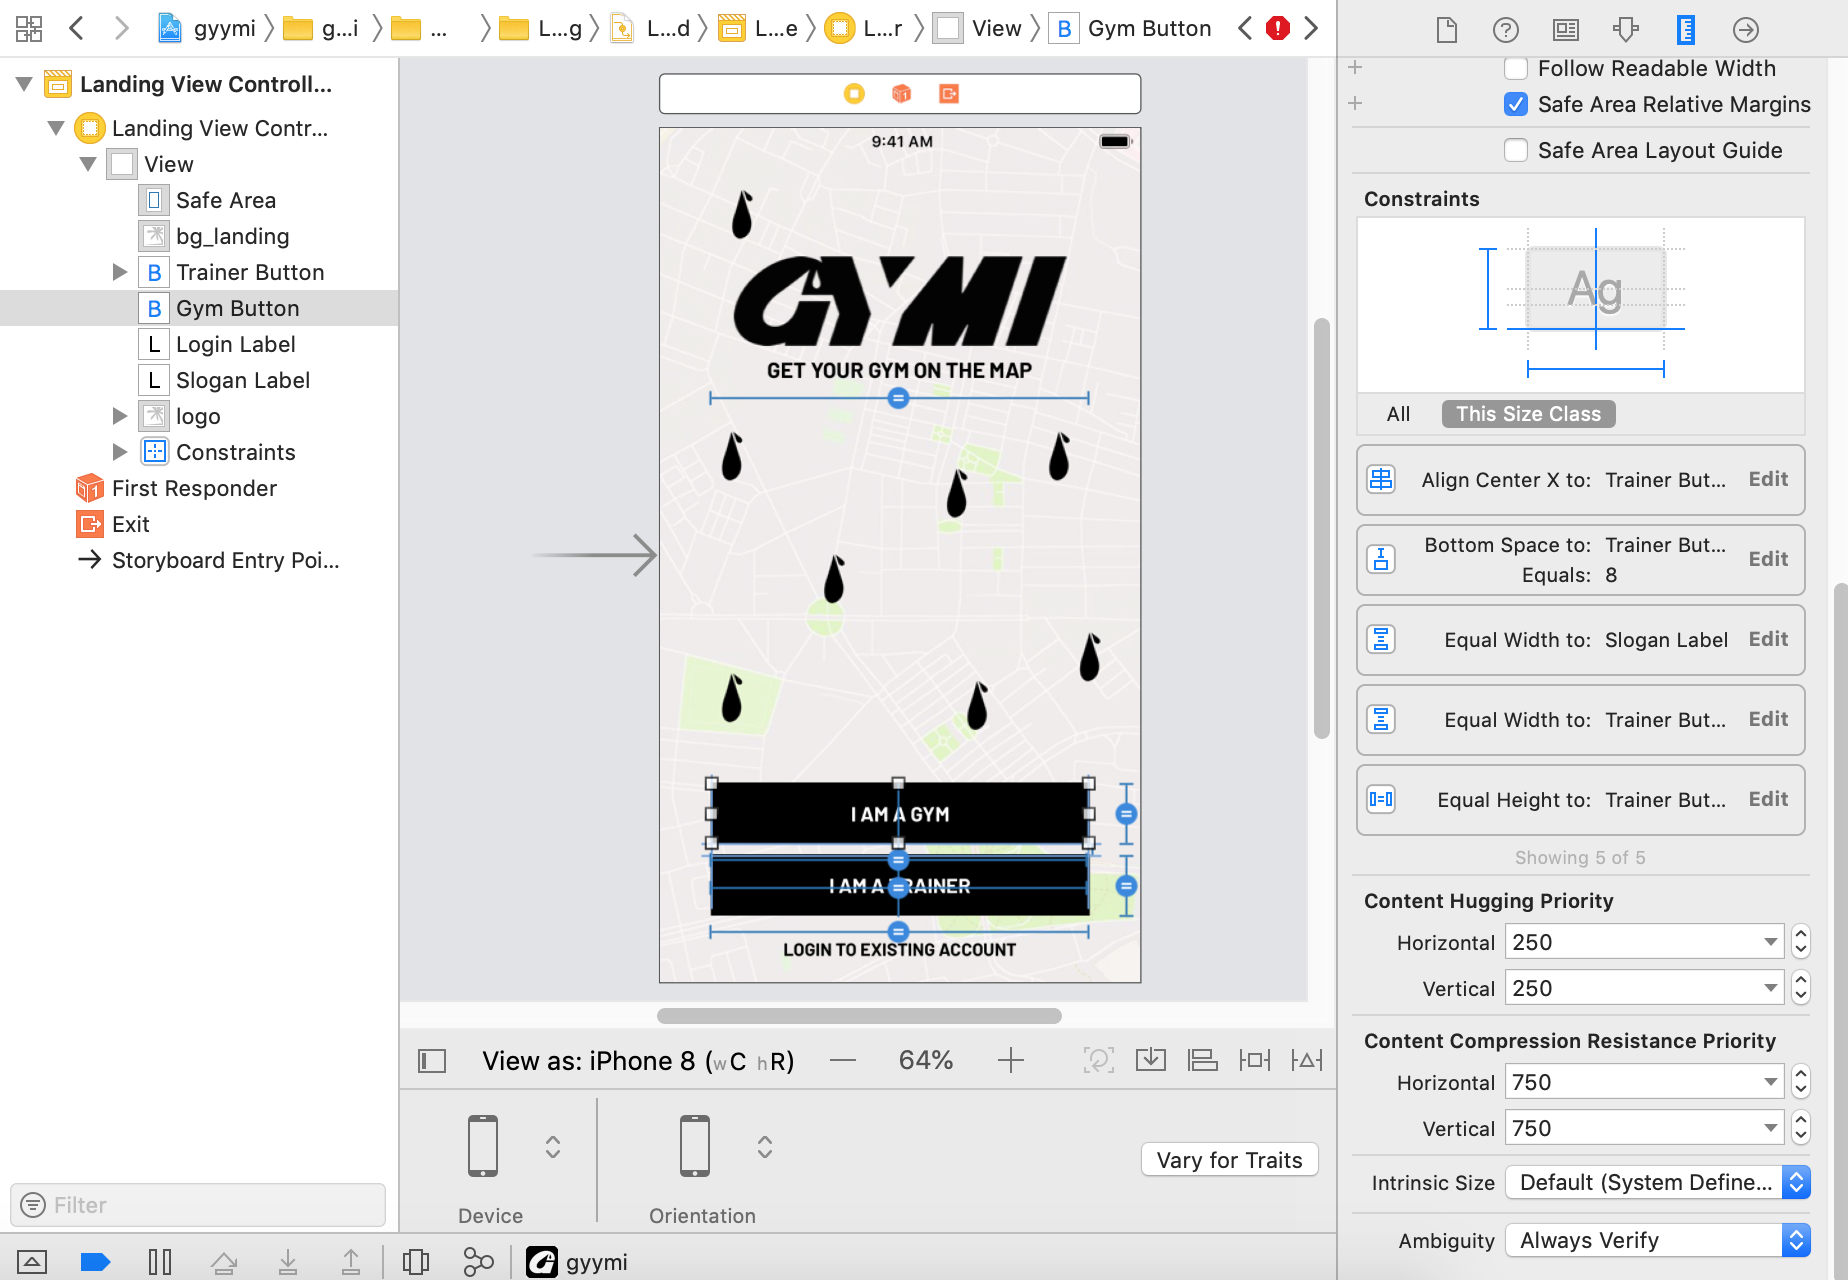
\includegraphics[width=0.8\textwidth]{pfc/figuras/storyboard.png}
    \caption{Uso de \textit{Storyboard}'s para implementação de interface gráfica}
    \label{fig:storyboard}
\end{figure}

\subsection{Critérios de Avaliação}
A implementação do aplicativo foi avaliada seguindo critérios técnicos para garantir a qualidade do produto e a conformidade com os requisitos do projeto. Alguns destes critérios e práticas adotadas para atendê-los são discutidos a seguir.

Em relação ao código, algumas abordagens foram estabelecidas para mantê-lo limpo, em conjunto com as boas práticas de programação. Foi utilizado a ferramenta \textit{SwiftLint} \cite{swift-lint} para assegurar a padronização de estilo e a conformidade com convenções estabelecidas para a escrita na linguagem Swift. Sempre que o código é compilado, avisos são gerados na IDE caso algum desvio de padrão seja encontrado no código. Boas práticas de programação também foram utilizadas para avaliar a qualidade do código, como a divisão de responsabilidades e reuso de componentes.

A avaliação da interface gráfica foi feita com base em testes de múltiplos dispositivos. Através da SDK iOS integrada ao Xcode, foi possível realizar a simulação do aplicativo em diferentes dispositivos. O critério utilizado para a aprovação de uma interface gráfica foi a avaliação positiva (conformidade com o projeto de design da aplicação e ausência de comportamentos gráficos estranhos) em pelo menos dois tipos de dispositivos de diferentes tamanhos de telas. A Figura \ref{fig:devices} ilustra o teste feito para a tela de dashboard das academias nos simuladores do iPhone SE, iPhone 7 e iPhone X.

\begin{figure}[H]
	\centering
    \begin{subfigure}[b]{0.3\textwidth}
        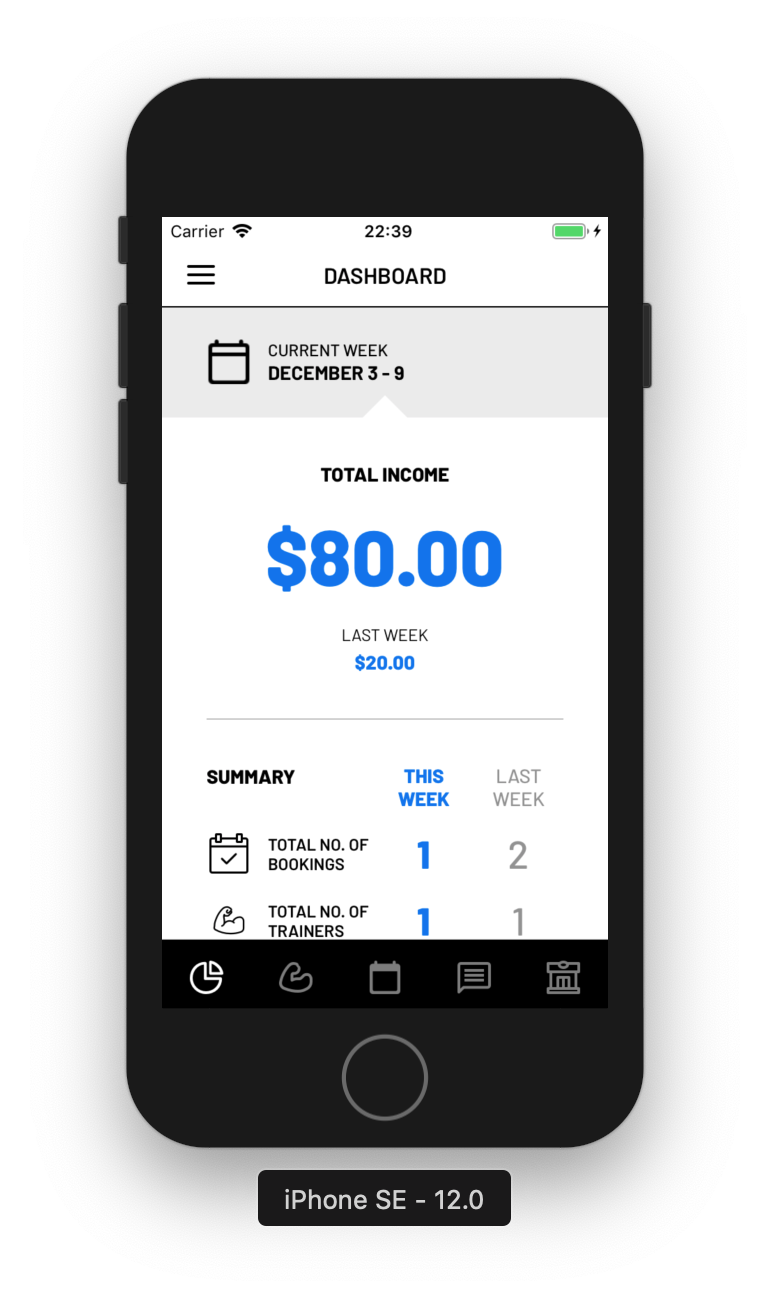
\includegraphics[width=\textwidth]{pfc/figuras/se.png}
        \caption{Simulador iPhone SE}
        \label{fig:se}
    \end{subfigure}
    ~
	\begin{subfigure}[b]{0.3\textwidth}
        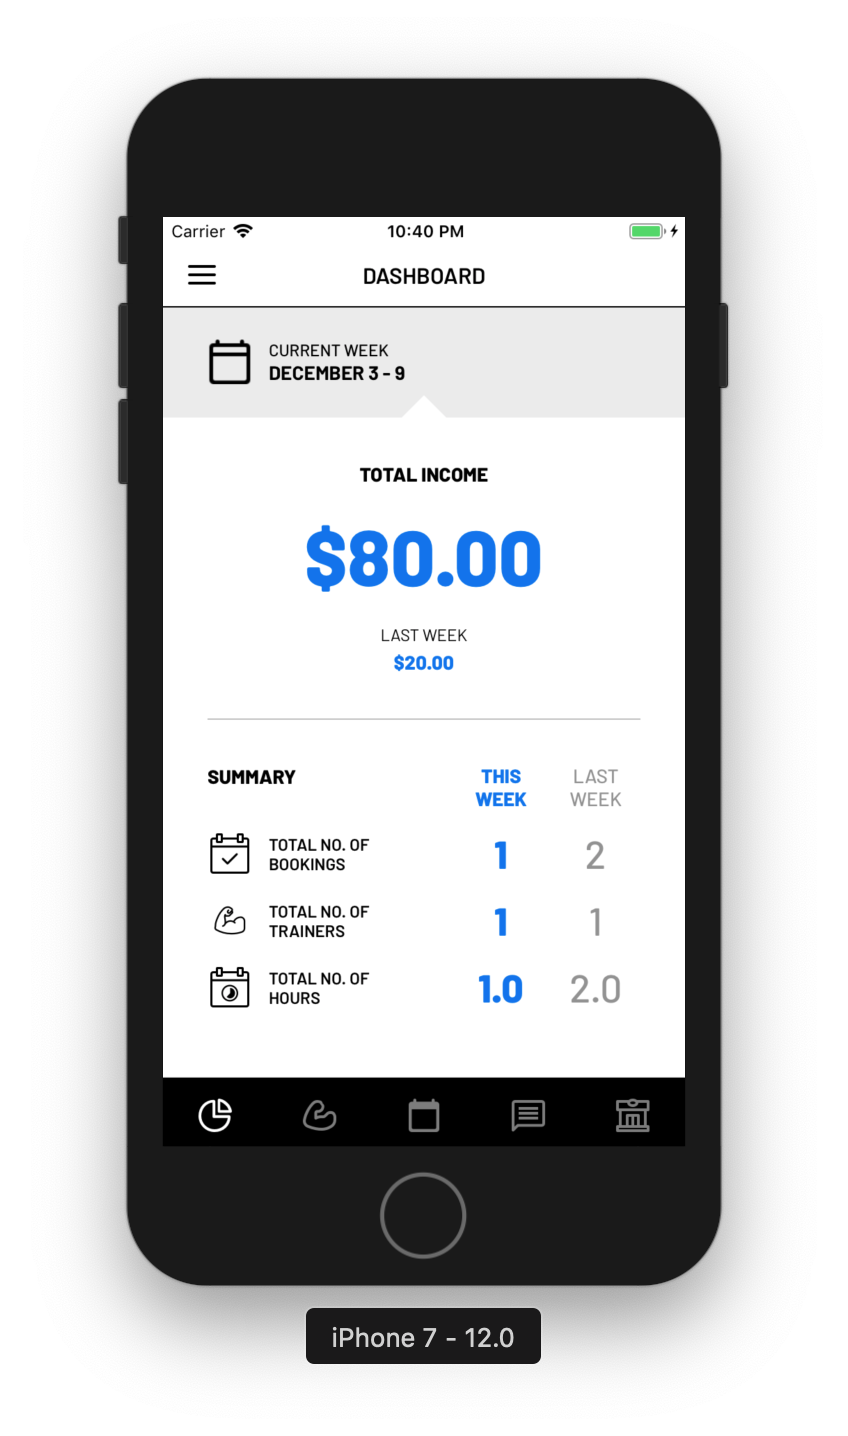
\includegraphics[width=\textwidth]{pfc/figuras/7.png}
        \caption{Simulador iPhone 7}
        \label{fig:7}
    \end{subfigure}
    ~
    \begin{subfigure}[b]{0.3\textwidth}
        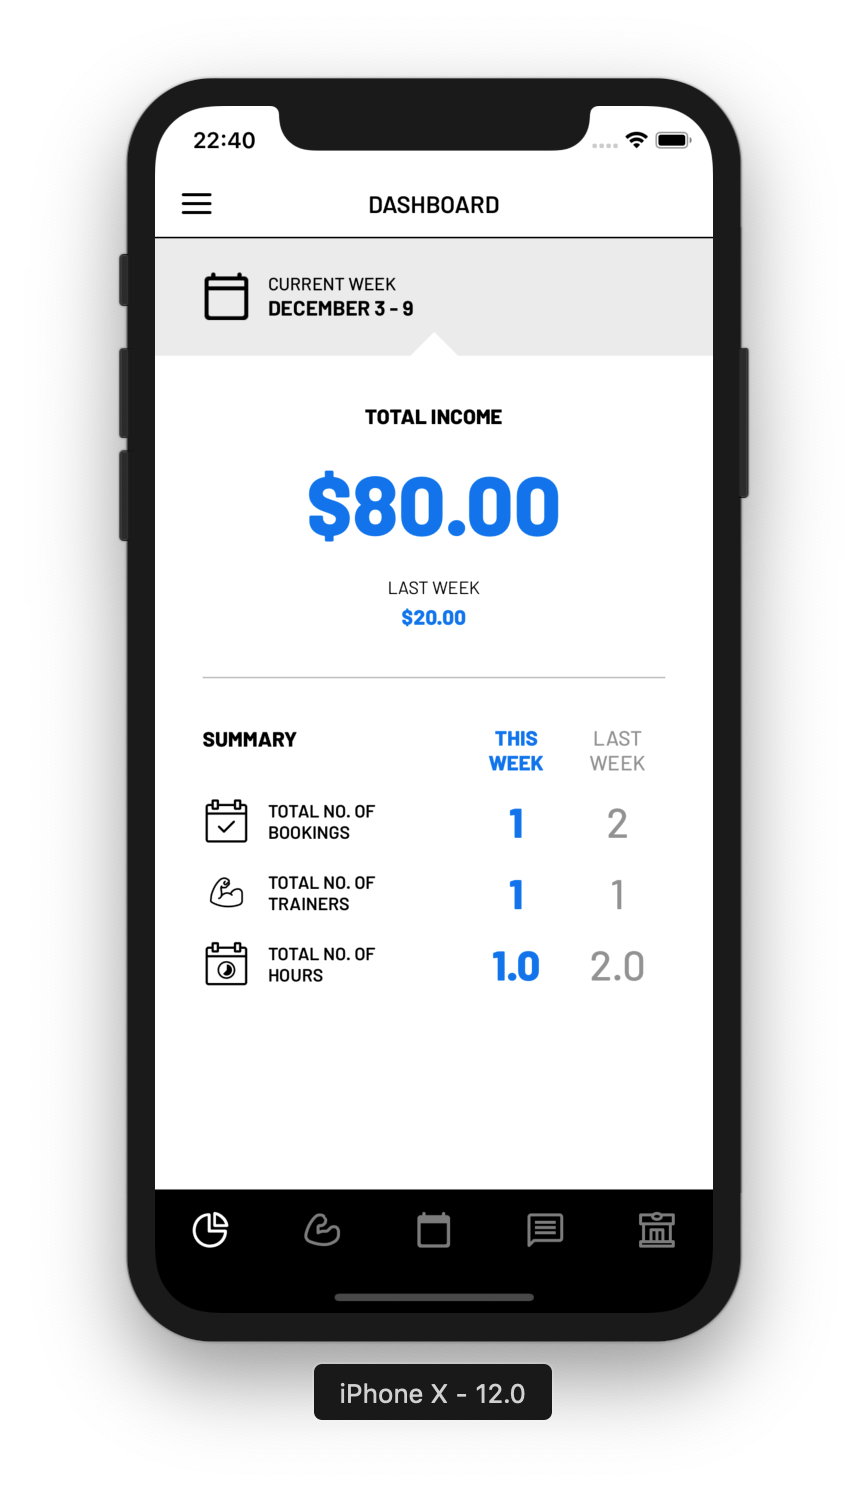
\includegraphics[width=\textwidth]{pfc/figuras/x.png}
        \caption{Simulador iPhone X}
        \label{fig:x}
    \end{subfigure}
    ~
    \caption{Uso de diferentes tipos de dispositivos}
    \label{fig:devices}
\end{figure}

\subsection{Desafios e Dificuldades de Implementação}
O desenvolvimento do aplicativo iOS apresentou alguns desafios de implementação, tanto lógicos como de interface gráfica. Alguns exemplos são apresentados a seguir.

Um dos desafios de implementação da interface gráfica do aplicativo foram as tabelas de horários e calendários (Figuras \ref{fig:gym-block}, \ref{fig:gym-booking-calendar}). A solução encontrada foi a utilização das bibliotecas \textit{SpreadsheetView} \cite{spreadsheet} e \textit{FSCalendar} \cite{fscalendar}, que forneceram componentes customizáveis para auxiliar o desenvolvimento.

Uma dificuldade recorrente em muitas das telas do aplicativo foi a adaptação dos elementos gráficos a diferentes tamanhos de dispositivos, principalmente aos menores aparelhos, como o iPhone SE. Essa dificuldade surgiu devido ao fato do design do projeto ter sido baseado em dispositivos maiores. Uma das soluções para alguns casos foi diferenciar o comportamento da tela baseado no tamanho do dispositivo, classificado como pequeno ou grande através de um método de auxílio.

Em relação à parte lógica do aplicativo, o tratamento de erros apresentou alguns desafios de implementação. Muitos casos de erros e validação de campos tiveram que ser tratados no momento do cadastro dos usuários (Figura \ref{fig:register-errors}). Um exemplo de solução implementada para a validação de campos foi a utilização de expressões regulares. Erros advindos de falhas nas chamadas de API's também demandaram tempo de projeto, como a falha de autenticação de usuário ilustrada na Figura \ref{fig:session-expired}, que ocorre quando o \textit{token} do usuário é inválido. Neste último caso, a solução implementada foi apresentar um aviso explicando o problema e, em seguida, forçar o logout no aplicativo.

\begin{figure}[H]
	\centering
    \begin{subfigure}[b]{0.4\textwidth}
        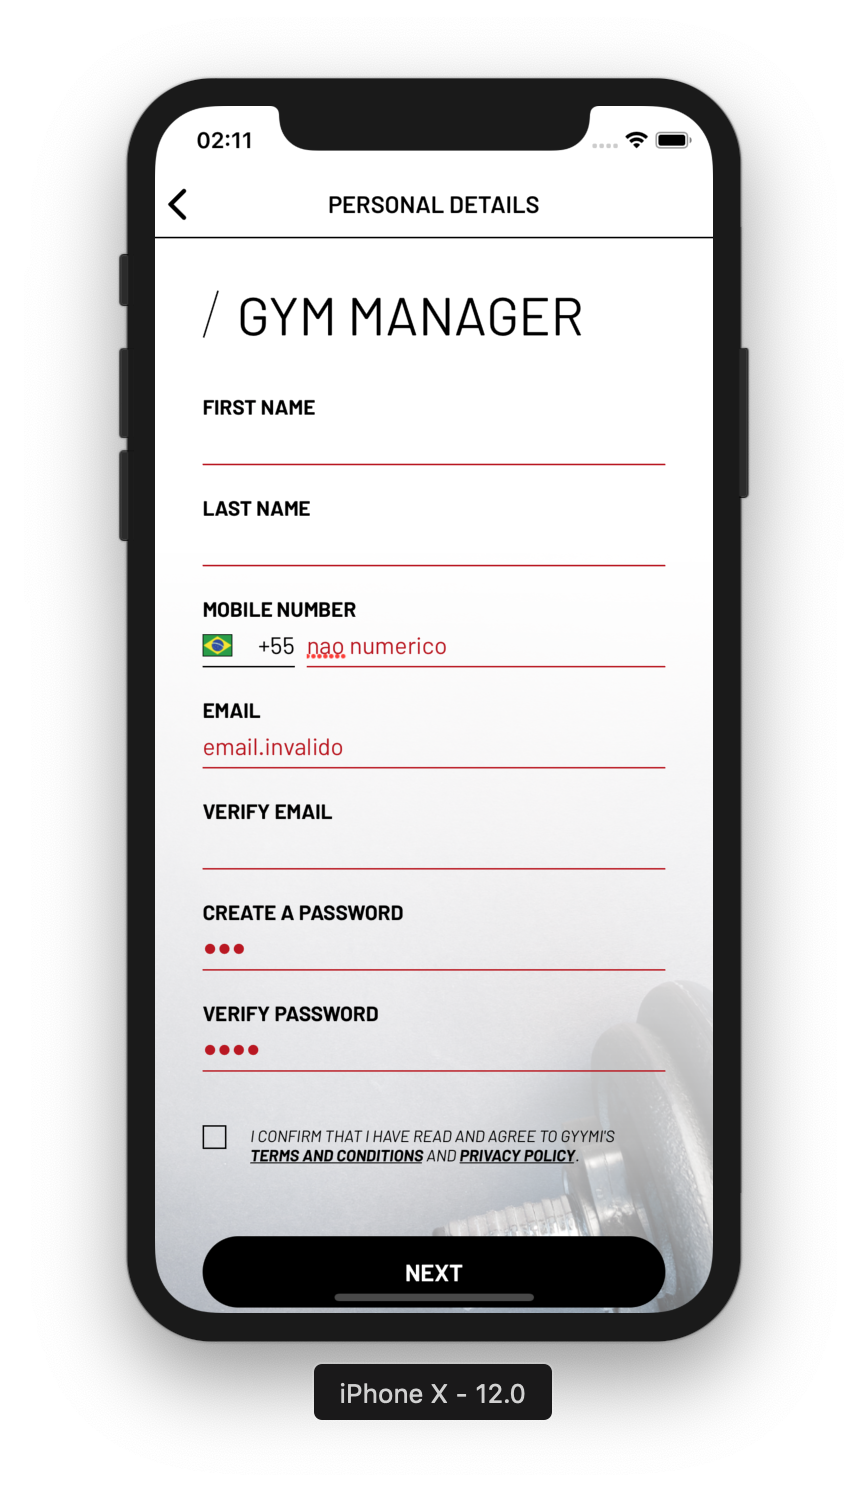
\includegraphics[width=\textwidth]{pfc/figuras/register-errors.png}
        \caption{Erros no cadastro}
        \label{fig:register-errors}
    \end{subfigure}
    ~
	\begin{subfigure}[b]{0.4\textwidth}
        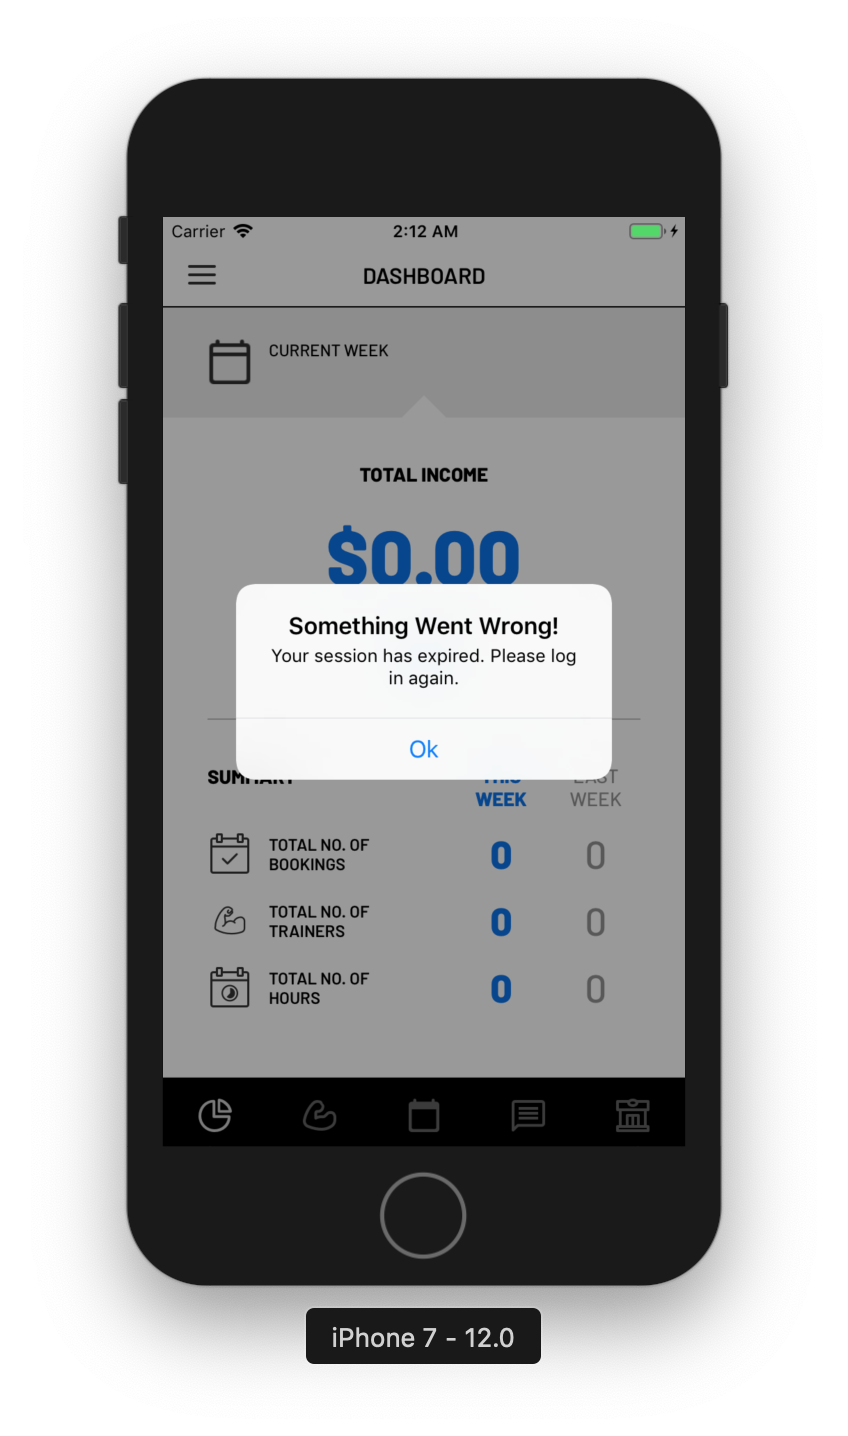
\includegraphics[width=\textwidth]{pfc/figuras/session-expired.png}
        \caption{Erro de autenticação}
        \label{fig:session-expired}
    \end{subfigure}
    ~
    \caption{Exemplos de estados de erro no aplicativo}
    \label{fig:error-states}
\end{figure}

% **********************
% Integração de Sistemas
% **********************
\section{Integração de Sistemas}
O desenvolvimento da aplicação evolveu a integração de múltiplos sistemas de software, tanto internos quanto externos. Nesta seção, primeiro é apresentada a integração com o sistema de back-end, desenvolvido internamente. Em seguida, o mesmo é feito para os sistemas externos. Por último, a ferramenta utilizada para testes das integrações feitas por RESTful API's são apresentadas. 

\subsection{Back-end}
A integração com o back-end foi feita por meio de uma API REST. A API fornece endpoints que retornam informações relacionadas à lógica de negócio da aplicação e permitem o cadastro de dados do usuário.

O formato utilizado para troca de dados foi o JSON (Figura \ref{fig:json}). Este formato foi utilizado por apresentar uma notação simples para entendimento e pelo fato de ser utilizado em larga escala em integrações de serviço web. Do ponto de vista humano, a notação é de fácil visualização por não apresentar uma sintaxe verbosa. Além disso, o formato tem suporte nativo de diversas linguagens de programação, incluindo o Swift, utilizado para realizar a implementação.

\begin{figure}[H]
    \centering
    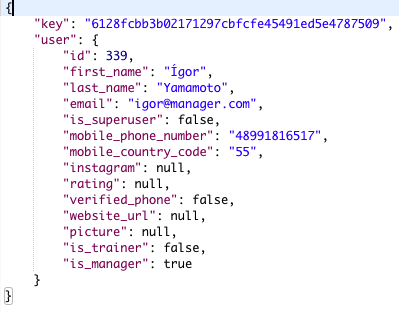
\includegraphics[width=0.8\textwidth]{pfc/figuras/json.png}
    \caption{Exemplo de resposta do back-end no formato JSON}
    \label{fig:json}
\end{figure}

A API contém algumas características relacionadas à segurança do sistema. A API fornece diferentes níveis de acesso para as chamadas a fim de proteger dados sensíveis. Todo usuário recebe um \textit{token} no momento em que realiza o login ou é registrado no aplicativo. Este \textit{token} é utilizado para realizar a autenticação de chamadas da API, permitindo a identificação do usuário que realizou a requisição pelo aplicativo. Através da identificação, o back-end pode retornar ou negar o pedido de chamada de API de acordo com o nível de acesso do usuário. Além da autenticação e autorização de usuários no sistema, existem dois ambientes de uso da API: um para fase de desenvolvimento e testes, outro para o aplicativo em produção. Ambos os ambientes contêm o mesmo conjunto de chamadas de API disponíveis, distinguindo-se apenas no uso de diferentes bancos de dados (desenvolvimento e produção). Este recurso permite a separação do uso do aplicativo para fins de testes, realizados pelo time de desenvolvimento e pelo cliente, e para fins de uso real, feito pelo usuário final. A separação dos ambientes é feita a partir da diferenciação da URL base da API REST.

No código do aplicativo, as chamadas de API são feitas com o auxílio de uma biblioteca para a linguagem Swift. A biblioteca, denominada Alamofire \cite{alamofire}, é uma camada de abstração para a utilização de recursos de rede do sistema iOS.

O recebimento dos dados da API é feita a partir de uma tradução automática do formato JSON para objetos do Swift. A tradução é feita através da utilização de recursos nativos do Swift. Além disso, é utilizado um parâmetro de configuração que transforma a notação \textit{snake case} da API para a notação \textit{camel case}, utilizada no código.

\subsection{Serviços Externos}
O desenvolvimento do aplicativo teve como requisito a implementação dos sistemas de geolocalização, pagamento e envio de SMS. No projeto, optou-se pela utilização destes sistemas na forma de serviços devido ao grande esforço envolvido na implementação e manutenção dos mesmos. Existem diversas alternativas consolidadas há anos no mercado para cada um dos sistemas citados. As soluções escolhidas e as integrações realizadas são apresentadas a seguir. 

\subsubsection{Geolocalização}
O aplicativo apresentou como um de seus requisitos funcionais a presença de um sistema de mapa, assim como a utilização da localização do usuário. Foi escolhido o serviço de geolocalização do Google Maps \cite{google-maps}, pelo motivo do mesmo disponibilizar uma SDK para o sistema iOS de fácil utilização, com boa documentação e suporte em comunidades da internet. Para detectar a localização do usuário, utilizou-se o recurso de GPS nativo do sistema iOS, disponibilizado através do framework \textit{Core Location}, parte da camada de \textit{Core Services} do sistema operacional.

O serviço de geolocalização do Google Maps é utilizado em diversas partes do aplicativo. No momento do cadastro de uma academia, o serviço é utilizado para o preenchimento do campo endereço (Figura \ref{fig:address-field}), obrigatório para todos os estabelecimentos cadastrados na plataforma. Requisições são feitas para a API do Google Maps à medida que o usuário acrescenta caracteres no campo de endereço. Como retorno, opções de endereços semelhantes ao digitado são apresentadas na interface (Figura \ref{fig:search-delfino}). Uma vez que o usuário escolhe um dos endereços disponíveis na busca, o serviço de geolocalização retorna as coordenadas referentes ao endereço. Estas coordenadas são enviadas ao back-end para armazenamento no banco de dados, junto aos demais dados da academia, e posteriormente são utilizadas para demarcação dos estabelecimentos no mapa.

\begin{figure}[H]
	\centering
    \begin{subfigure}[b]{0.4\textwidth}
        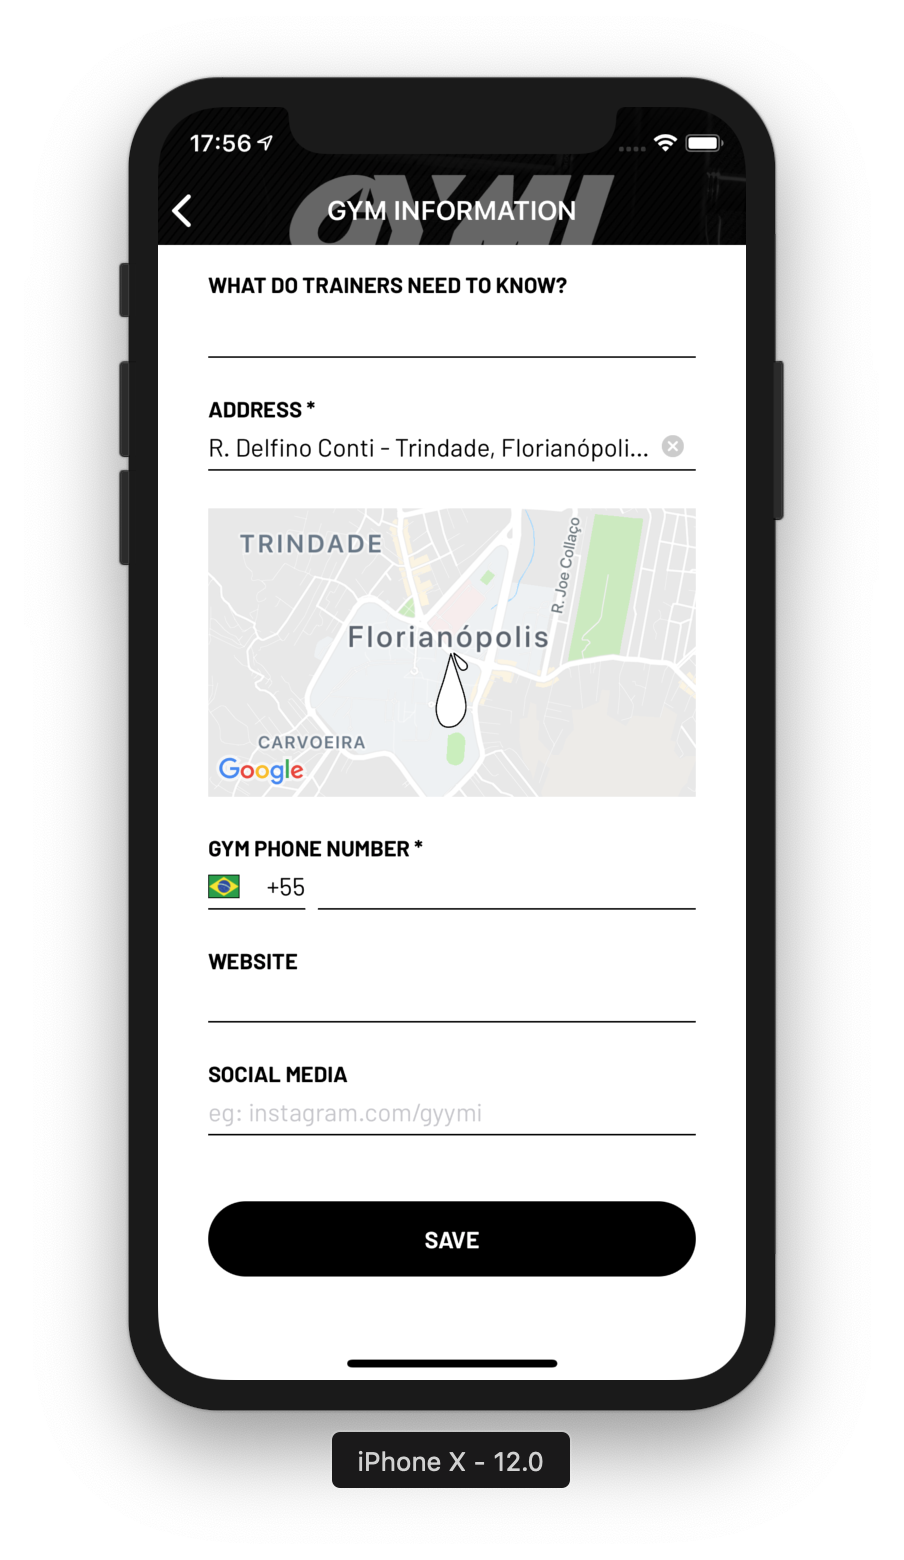
\includegraphics[width=\textwidth]{pfc/figuras/delfino-conti-2.png}
        \caption{Preenchimento do campo de endereço}
        \label{fig:address-field}
    \end{subfigure}
    ~
	\begin{subfigure}[b]{0.4\textwidth}
        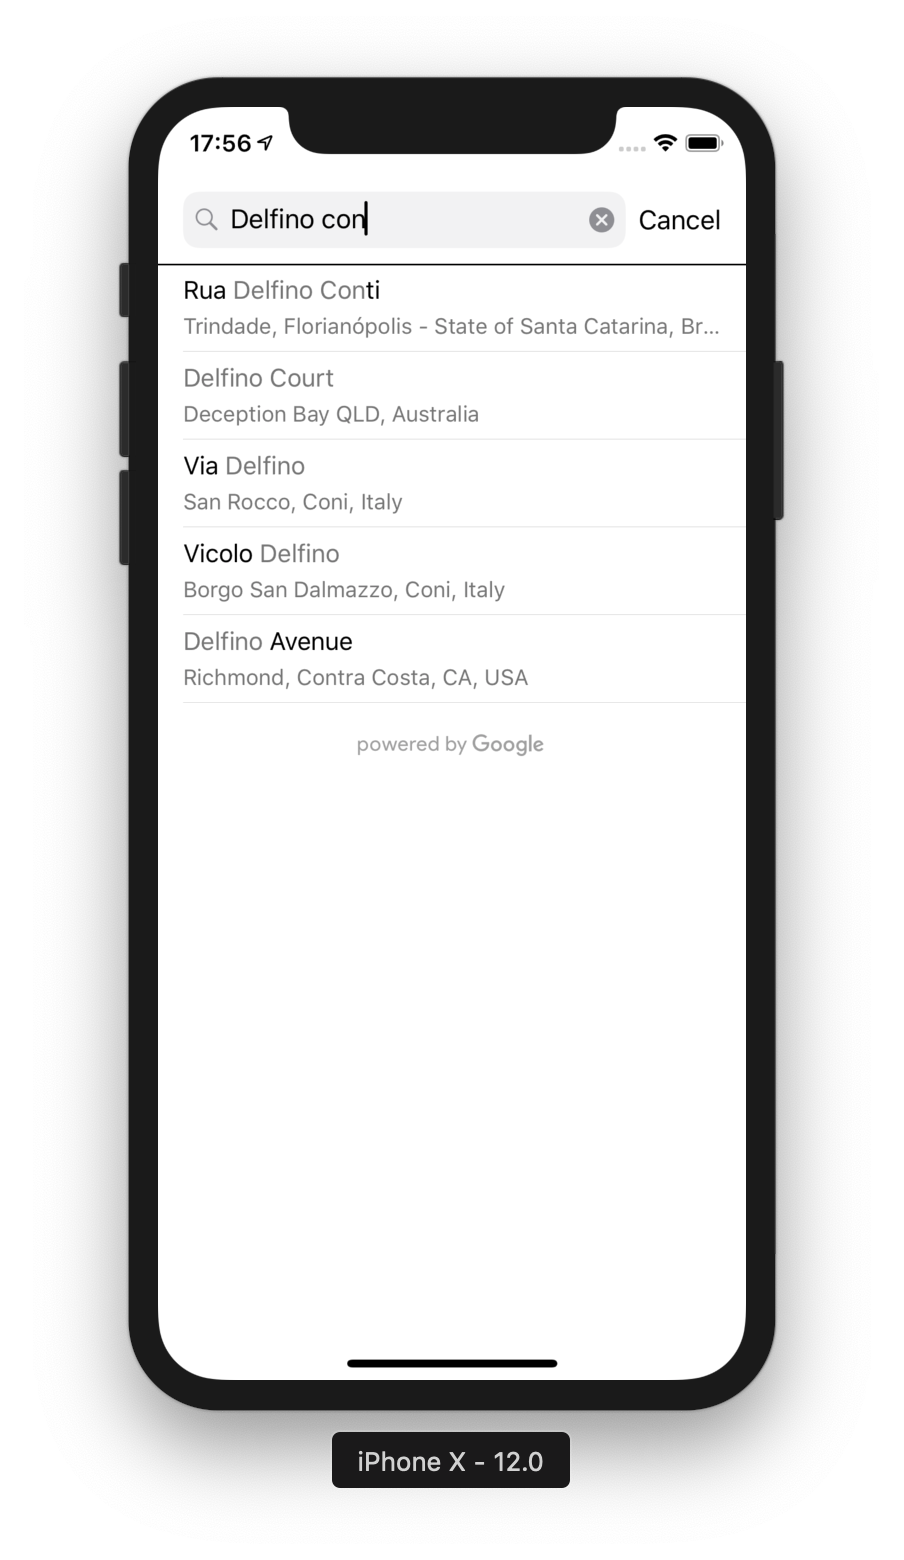
\includegraphics[width=\textwidth]{pfc/figuras/delfino-conti.png}
        \caption{Busca por endereços através da API do Google Maps}
        \label{fig:search-delfino}
    \end{subfigure}
    ~
    \caption{Etapa de preenchimento do campo endereço no cadastro de uma academia}
    \label{fig:addreess-field-fill}
\end{figure}

Outra utilização do serviço de geolocalização é o sistema de mapas, recorrente em diversas telas do aplicativo. O sistema de mapas é utilizado de maneira estática (sem a interação do usuário) nas telas de boas vindas (Figura \ref{fig:gym-welcome}), de perfil (Figuras \ref{fig:gym-profile} e \ref{fig:tr-gym-profile-view}) e de cadastro (Figura \ref{fig:address-field}) das academias e, também, na tela de confirmação de agendamento de treino (Figura \ref{fig:tr-booking-confirmed}). Na interface do treinador (Figura \ref{fig:tr-gym-search}), o mapa é renderizado na tela dinamicamente conforme a interação do usuário. O sistema de mapas permite a utilização de movimentos de pinça para alterar o zoom, além da movimentação simples do mapa através de toques na tela. Sempre que um mapa é renderizado na tela do aplicativo, uma requisição é feita ao back-end a fim de identificar as academias que estão presentes naquela região do mapa. O ponto central da região do mapa é enviado junto com um raio de busca (foi utilizado como padrão um raio de busca de $5\,km$) para o back-end. Então, uma lista com todas as academias da região é retornada e, a partir dos dados de coordenadas salvos, marcações são feitas no mapa.
                               
O framework \textit{Core Location} é utilizado em conjunto com o sistema de mapas para detectar a posição atual do usuário. Para utilizar o recurso nativo do sistema iOS, uma requisição de permissão de uso do sistema de localização do dispositivo deve ser feita ao usuário (Figura \ref{fig:gps-permission}). Em seguida, uma marcação especial é feita no mapa (ícone de músculos do braço - Figura \ref{fig:muscle-marker}) para indicar a localização corrente. A partir deste instante, um observador é configurado para que o sistema operacional emita um aviso ao aplicativo quando o usuário se movimentar. A configuração é feita com um parâmetro de precisão de $10/,m$. Assim, quando o usuário se desloca mais que esta distância, um aviso é emitido ao aplicativo e, em seguida, a posição do marcador no mapa é atualizada.

\begin{figure}[H]
	\centering
    \begin{subfigure}[b]{0.38\textwidth}
        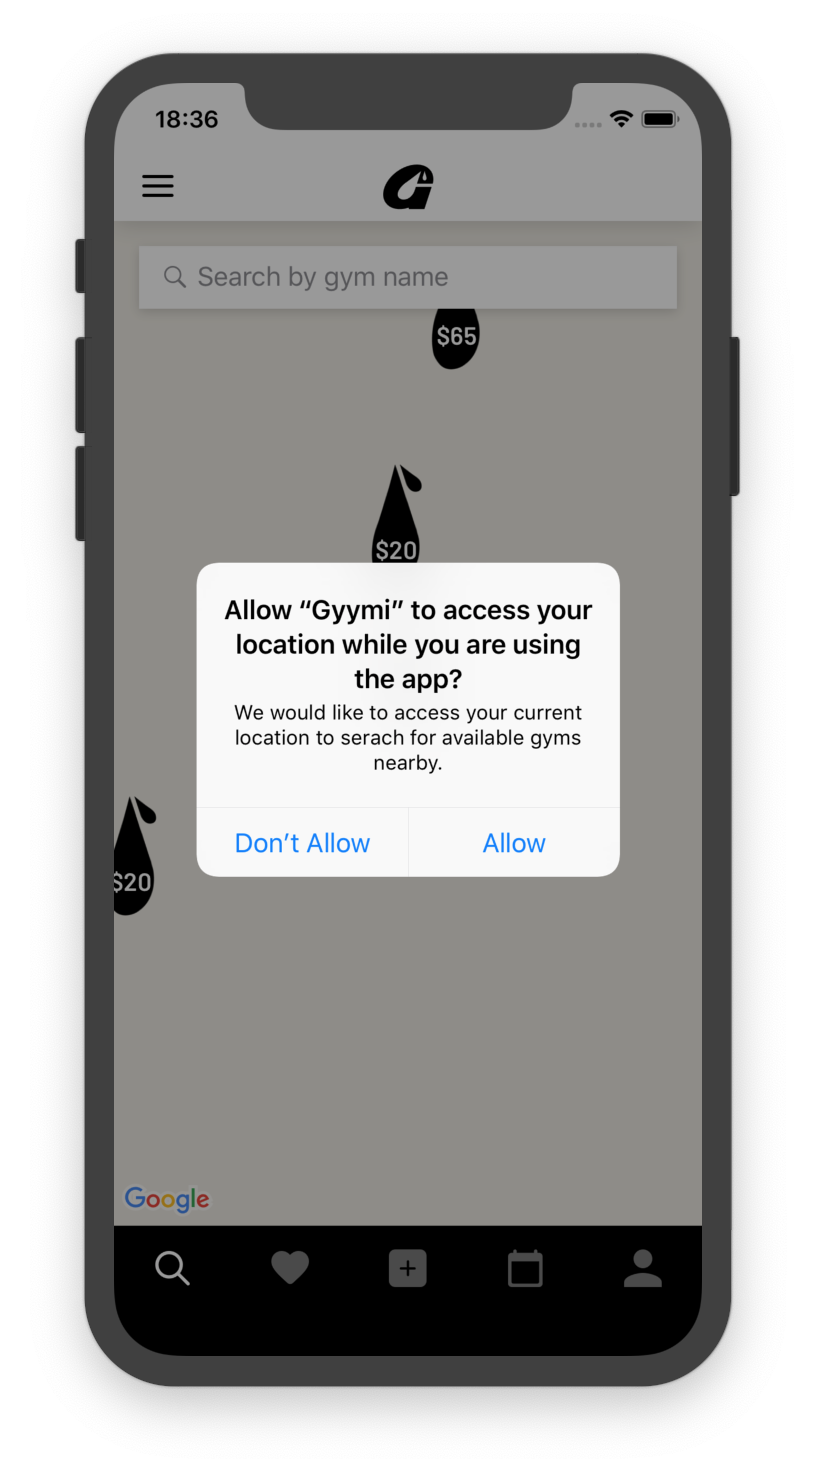
\includegraphics[width=\textwidth]{pfc/figuras/gps-permission.png}
        \caption{Permissão de uso do GPS}
        \label{fig:gps-permission}
    \end{subfigure}
    ~
	\begin{subfigure}[b]{0.4\textwidth}
        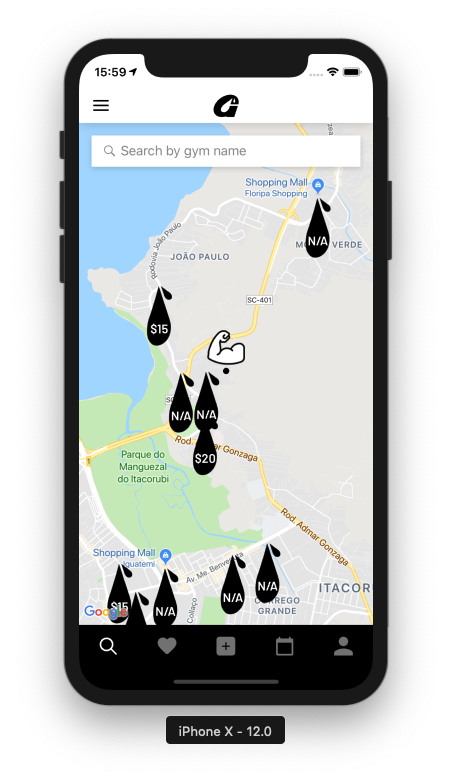
\includegraphics[width=\textwidth]{pfc/figuras/tr-home.png}
        \caption{Marcador de posição}
        \label{fig:muscle-marker}
    \end{subfigure}
    ~
    \caption{Marcação da posição atual do usuário no mapa}
    \label{fig:user-position}
\end{figure}

\subsubsection{Pagamento}
Um sistema de pagamentos foi utilizado para que as transações financeiras possam ocorrer dentro da plataforma. O serviço escolhido para implementação desta funcionalidade foi o Stripe \cite{stripe}. O serviço foi escolhido por apresentar a melhor usabilidade do ponto de vista de desenvolvimento, apresentando uma boa documentação e estrutura de API's e disponibilização de SDK para iOS com diversos recursos embutidos, como validação de campos de cartão de crédito.

O funcionamento do sistema de pagamentos da aplicação é ilustrado na Figura \ref{fig:payment-system}. Por questões de segurança, nenhum dado sensível (como número do cartão de crédito ou conta bancária) é armazenado no banco de dados da aplicação. Esta tarefa é delegada ao Stripe, assim como a realização de todas as transações financeiras. Na plataforma do Stripe, são criadas contas virtuais para cada academia, assim como uma conta virtual do Gyymi. Além disso, um processo de \textit{tokenização} é feito para a representação dos cartões de crédito dos treinadores. A \textit{tokenização} funciona da seguinte forma (ver Figura \ref{fig:seq-diagram-token}): o usuário informa os dados do cartão através da interface gráfica do aplicativo iOS; os dados são enviados para o Stripe, onde são armazenados; um \textit{token} de identificação única para representar o cartão de crédito é gerado e enviado ao aplicativo iOS; o \textit{token} é enviado ao back-end, que após validar o mesmo com o Stripe, armazena-o no banco de dados da aplicação; por último, o back-end retorna uma resposta ao aplicativo iOS informando que o processo de \textit{tokenização} do cartão de crédito foi concluído com sucesso. Dessa forma, a aplicação pode identificar cartões de crédito cadastrados e, em sequência, emitir pedidos de transação com o uso do \textit{token}.

Existem três tipos de transações dentro do Stripe:
\begin{itemize}
    \item Cobrança: quando um pagamento é feito pelo treinador, o Stripe emite uma cobrança no cartão de crédito cadastrado.
    \item Transferência: diz respeito as transferências entre contas virtuais do Stripe. Todos os pagamentos emitidos são enviados primeiramente à conta virtual do Gyymi, que retira uma taxa do pagamento como forma de cobrança pelo serviço de intermédio e, então, repassa o restante do valor para as contas virtuais das academias.
    \item Pagamento: ao final de um intervalo de tempo pré-definido, o dinheiro das contas virtuais é repassado para as contas bancárias reais.
\end{itemize}

\begin{figure}[H]
    \centering
    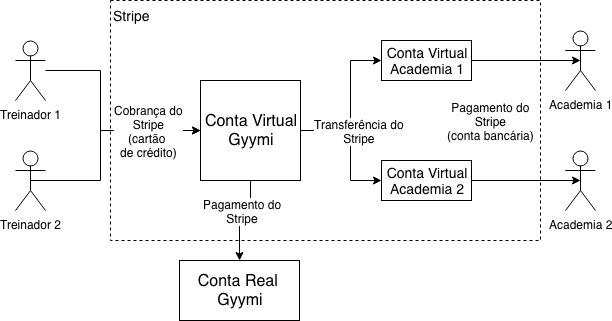
\includegraphics[width=0.8\textwidth]{pfc/figuras/payment-system-stripe.png}
    \caption{Funcionamento do sistema de pagamentos}
    \label{fig:payment-system}
\end{figure}

\begin{figure}[H]
    \centering
    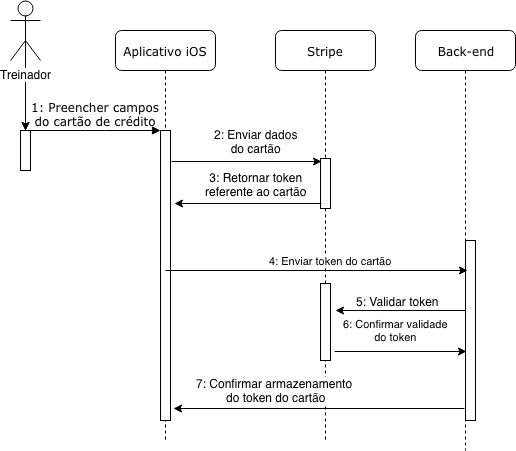
\includegraphics[width=0.8\textwidth]{pfc/figuras/seq-diagram-token.png}
    \caption{Diagrama de sequência da dinâmica de \textit{tokenização} do cartão de crédito}
    \label{fig:seq-diagram-token}
\end{figure}

A implementação dos esquemas apresentados não foi concluída para a fase piloto do aplicativo. Para o piloto, foi utilizado um ambiente fictício que o Stripe fornece para testes. Transações fictícias foram criadas no Stripe ao final dos agendamentos de treinos, emitindo-se cobranças em cartões de crédito fictícios.

\subsubsection{Envio de SMS}
O sistema de envio de SMS foi utilizado para cumprir o requisito funcional de envio de SMS para verificação de número telefônico. A verificação é feita somente no cadsatro de novos treinadores (Figura \ref{fig:register-trainer-verification}). O serviço utilizado foi o Twilio \cite{twilio}.

A dinâmica de envio de SMS é ilustrada no diagrama de sequência da Figura \ref{fig:seq-diagram-sms}. O sistema opera da seguinte forma: o usuário preenche o cadastro através da interface gráfica do aplicativo iOS, em especial o campo de número do celular; os dados de cadastro são enviados e validados no back-end, que faz uma chamada de API para o Twilio com um pedido de envio de SMS para o número de celular cadastrado; o usuário, então, preenche o campo de código de verificação no aplicativo com o código recebido via SMS; o código de verificação é enviado ao back-end, que realiza a validação do mesmo com o Twilio; por fim, uma confirmação da validação do código de verificação é enviada ao aplicativo iOS, permitindo que o usuário prossiga com o cadastro.

\begin{figure}[H]
    \centering
    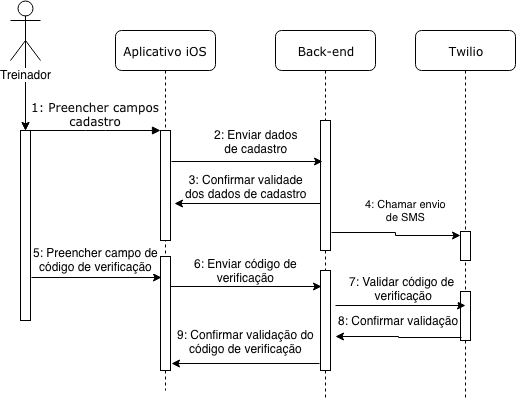
\includegraphics[width=0.8\textwidth]{pfc/figuras/seq-diagram-sms.png}
    \caption{Diagrama de sequência da dinâmica de envio de SMS para verificação de número telefônico}
    \label{fig:seq-diagram-sms}
\end{figure}

\subsection{Testes de RESTful API's}
Todas as integrações de sistemas apresentadas anteriormente foram realizadas utilizando RESTful API's. Com o intuito de agilizar e automatizar o processo de teste de chamadas de API, utilizou-se durante o projeto a ferramenta de software denominada Postman \cite{postman}. A ferramenta permite que conjuntos de chamadas de API's (coleções) sejam criadas, permitindo o teste das chamadas individualmente ou em conjunto (com o sequenciamento das chamadas).

A Figura \ref{fig:postman} ilustra a interface do Postman. Na esquerda, encontram-se as coleções, com as respectivas listas de chamadas de API. Na parte central superior, existem abas com as chamadas e seus parâmetros de configurações. Na parte central inferior, encontra-se um console onde a resposta da chamada é exibida.

\begin{figure}[H]
    \centering
    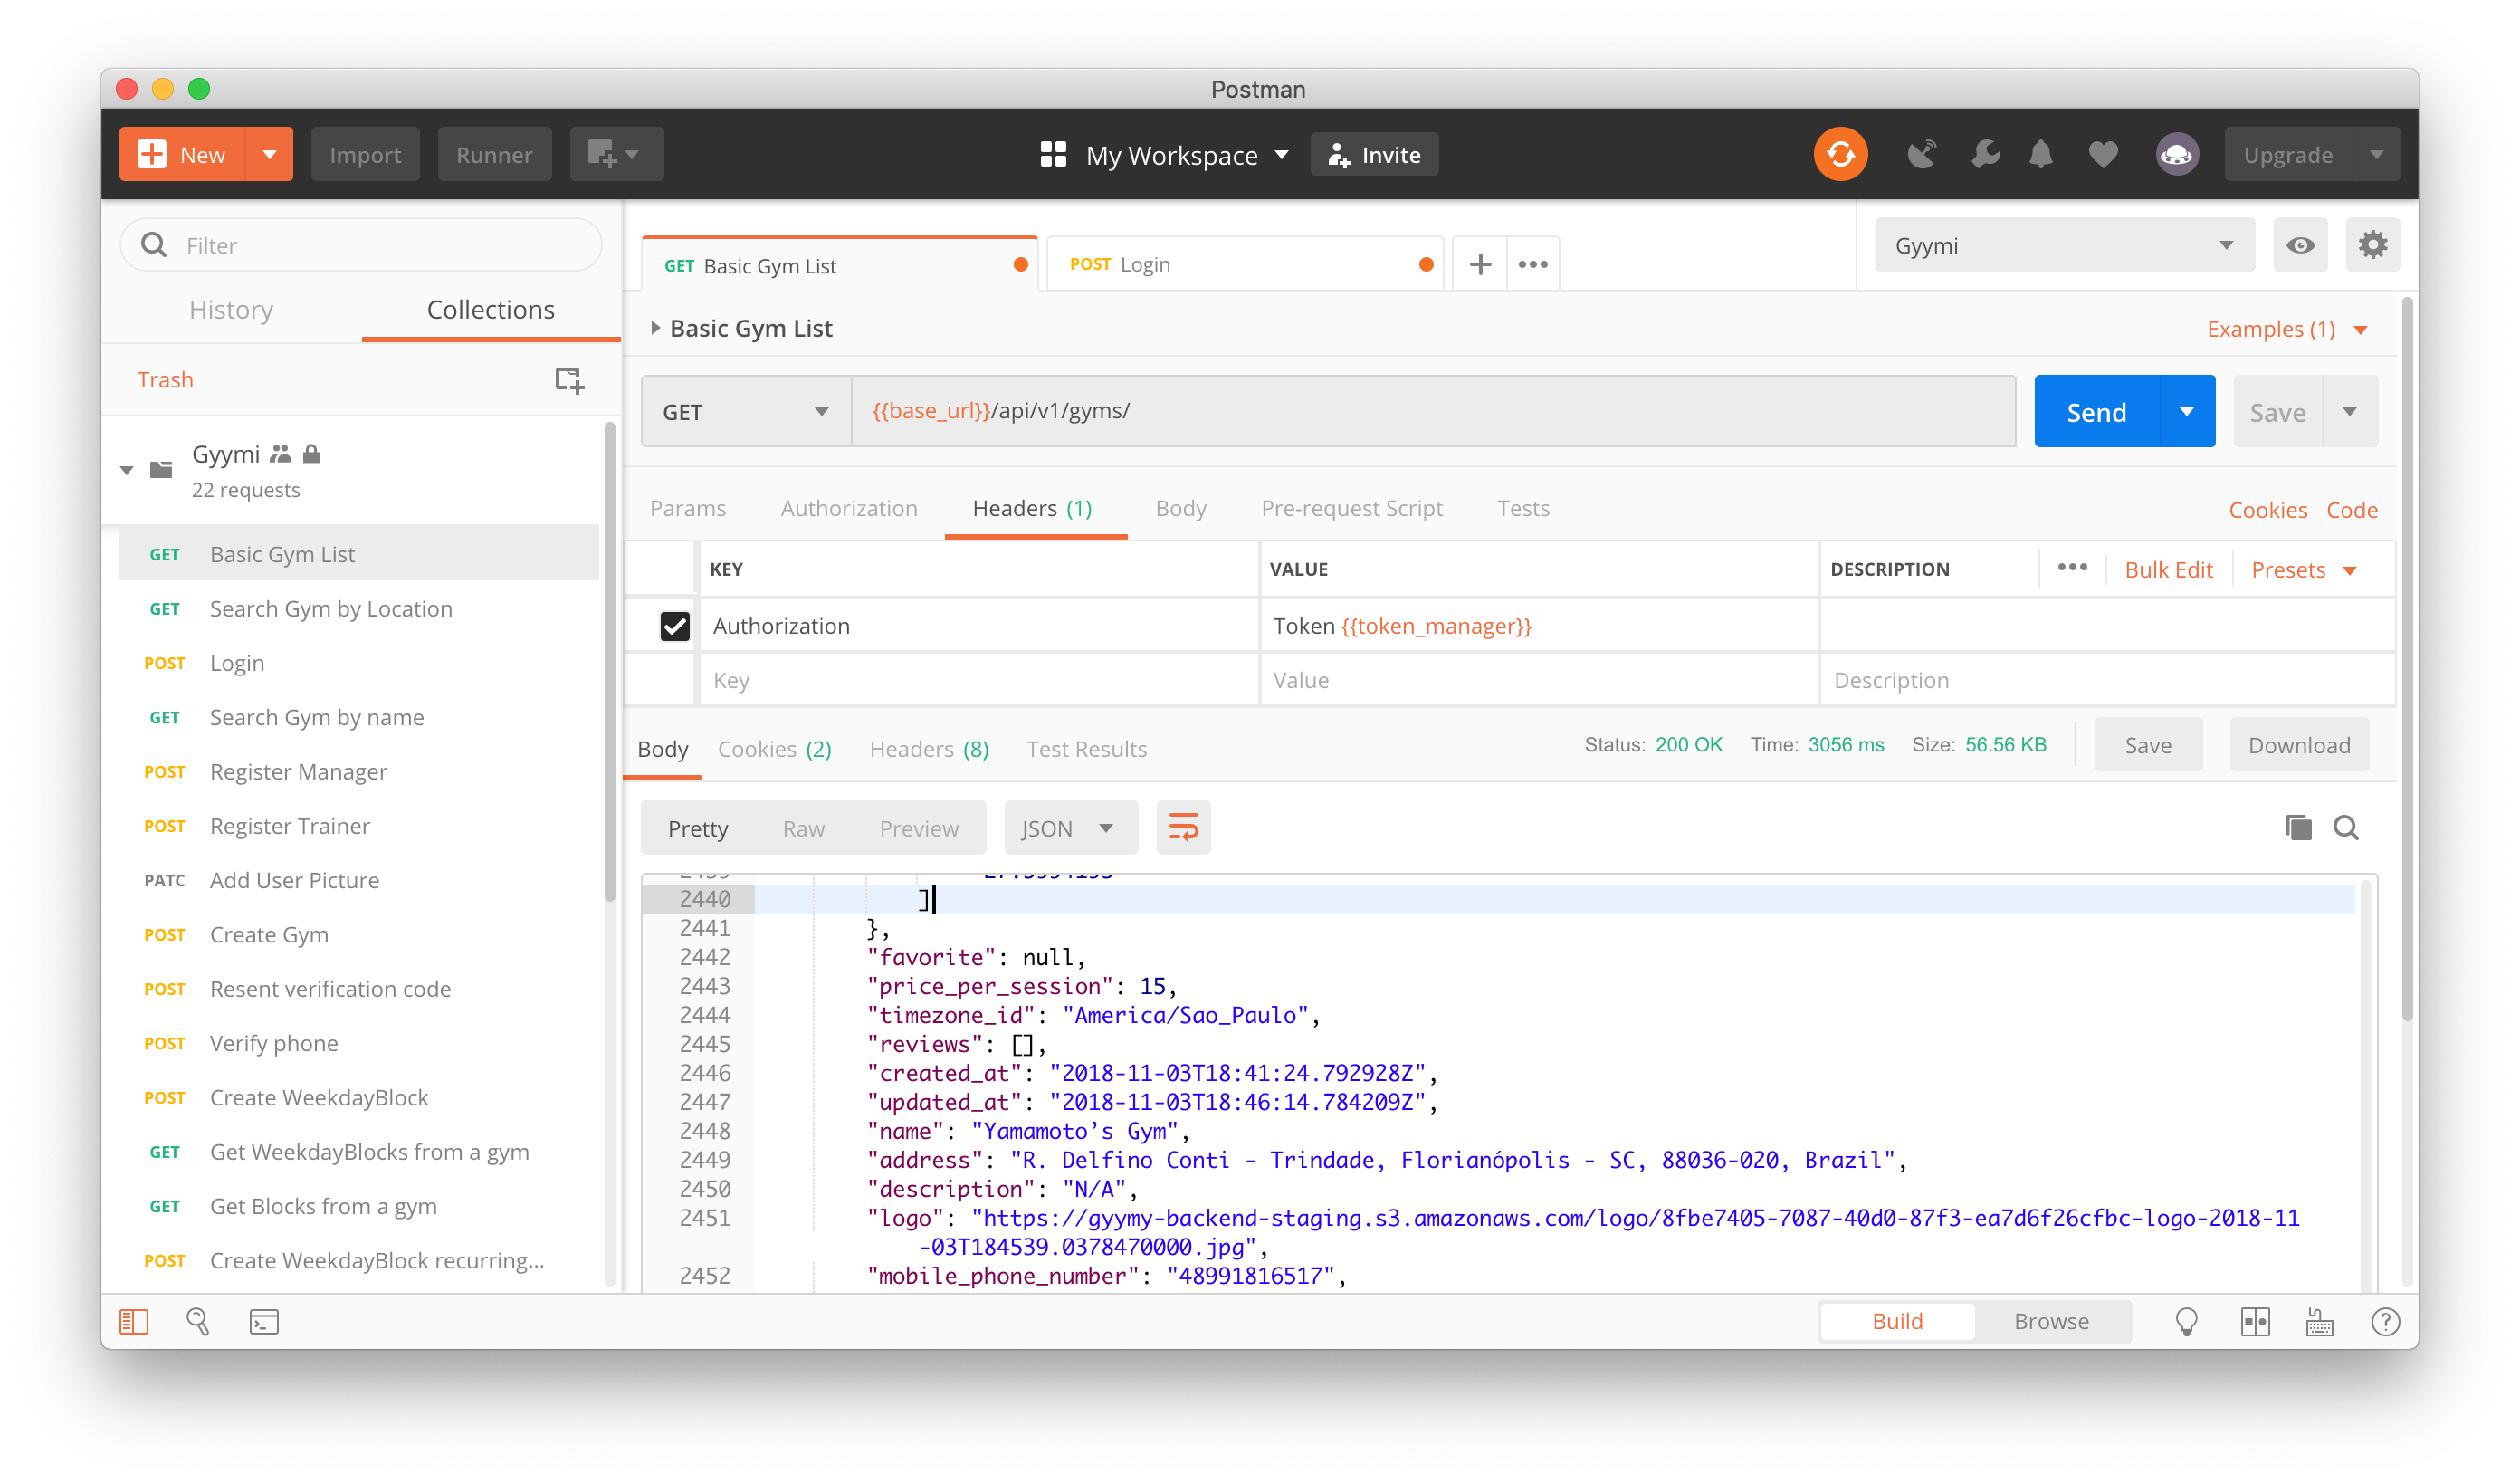
\includegraphics[width=0.8\textwidth]{pfc/figuras/postman.png}
    \caption{Postman - ferramente utilizada para testes de RESTful API's}
    \label{fig:postman}
\end{figure}

\chapter{Testes Automatizados de Interface Gráfica} \label{cap:tests}

\section{Definição do Projeto de Testes}
O projeto de testes da aplicação inicialmente previa apenas testes manuais, tanto a nível de código, quanto em relação à interface gráfica. Atualmente, a empresa Jungle Devs não tem uma estrutura formalizada para a implementação de testes automatizados em seus projetos de software. Testes manuais são realizados a cada final de \textit{sprint} por um time de garantia de qualidade, responsável por detectar problemas no sistema e por reportar os mesmos ao time de desenvolvimento.

O presente trabalho apresentou oportunidades para o início de um processo de estudo e implementação de testes automatizados dentro da empresa. Testes automatizados de interface gráfica podem ser realizados sem alterar a estrutura do software e o fluxo de trabalho da empresa. Esta característica se deve ao fato de se tratarem de testes do tipo caixa preta. Assim, optou-se por iniciar um projeto de testes experimental, a nível de interface gráfica, para avaliar possibilidades de adoção de testes automatizados dentro da empresa e a factibilidade do uso de ferramentas para este fim.

Os testes automatizados foram realizados com a interface do aplicativo já implementada. Como consequência, o projeto de testes teve início após o encerramento do ciclo de desenvolvimento da fase piloto do aplicativo. Assim, os testes foram tratados de forma isolada ao projeto do aplicativo, utilizando-se do mesmo apenas como cenário para um caso de estudo. Coube ao autor a responsabilidade completa pela condução do estudo dos testes.

A camada de testes automatizados de interface gráfica procura simular o comportamento do usuário final da aplicação. Assim, testes de aceitação são ideias para serem implementados neste nível. Dois casos de teste foram escolhidos para o estudo: fluxo de cadastro das academias e erros de cadastro do treinador. Ambos os casos pertencem a parte de cadastro do aplicativo. Estes foram escolhidos por se tratarem de cenários muito recorrentes em projetos de aplicativos, assim futuras implementações dentro da empresa podem se beneficiar deste trabalho.

\section{Ferramentas Escolhidas}
Os testes automatizados foram implementados com o auxílio de ferramentas específicas para este tipo de testes. Existem muitas opções de frameworks disponíveis, tanto proprietárias, quanto de código aberto. Neste projeto, optou-se pelo uso somente de ferramentas de código aberto, por serem de fácil acesso e terem bom suporte oferecido pela comunidade de software (desenvolvedores independentes e empresas).

Existem ferramentas com suporte específico para determinadas plataformas e outras que podem servir casos para múltiplas delas. O desenvolvimento do aplicativo Gyymi foi requisitado para duas plataformas: Android e iOS. Assim, um ferramenta que suportasse diferentes sistemas operacionais foi escolhida, o Appium. E devido ao fato do aplicativo apresentado neste trabalho ser voltado ao sistema iOS, outra ferramenta específica para a plataforma em questão também foi selecionada, o EarlGrey.

Além do Appium e do EarlGrey, também foi considerado a utilização da suíte de testes integrada ao Xcode, denominada XCUITest. Porém nenhum dos casos de teste implementados utilizou o XCUITest, pelo fato do desenvolvimento com o EarlGrey ser julgado suficiente para contemplar o uso de ferramentas específicas de plataforma. A ferramenta Appium foi a mais utilizada por apresentar maior potencial de reuso, tendo os dois casos de teste sido implementados com a mesma. O EarlGrey foi utilizado apenas no primeiro cenário de testes.

\section{Pré-configurações e Setup das Ferramentas}

\subsection{Modificações no Projeto}
A estrutura do código fonte do projeto manteve-se inalterada, contudo algumas adaptações foram realizadas para permitir as implementações. Os testes de interface gráfica foram desenvolvidos de modo a reconhecer componentes através da identificação de acessibilidade. Estas identificações não haviam sido criadas na fase de desenvolvimento do piloto e, portanto, tiveram que ser adicionadas aos componentes da interface que foram utilizados nos casos de teste.

\subsection{Appium}
A utilização do Appium foi feita através da API disponível para a linguagem Python. A escolha da linguagem se deve ao fato do autor já estar familiarizado com sua sintaxe e, também, pela empresa utilizar a linguagem em outras stacks, como no back-end. O código em Python foi escrito com editor de text Visual Studio Code.

Além da API em python, o Appium necessita que um servidor web local seja instanciado. Este é responsável por intermediar as interações entre os comandos enviados da API e o dispositivo móvel que contém o aplicativo. Para que este servidor seja criado, existem duas alternativas: através da CLI do Appium (Figura \ref{fig:appium-cli}) ou pela GUI do Appium (\ref{fig:appium-desktop}). As duas opções foram testadas. A CLI é de fácil utilização, contendo apenas um comando principal. A GUI oferece opções de configurações mais acessíveis, além de outras funcionalidades, como a inspeção (Figura \ref{fig:appium-desktop-inspector}) da execução do aplicativo (permite a visualização da hierarquia dos componentes da interface).

\begin{figure}[H]
    \centering
    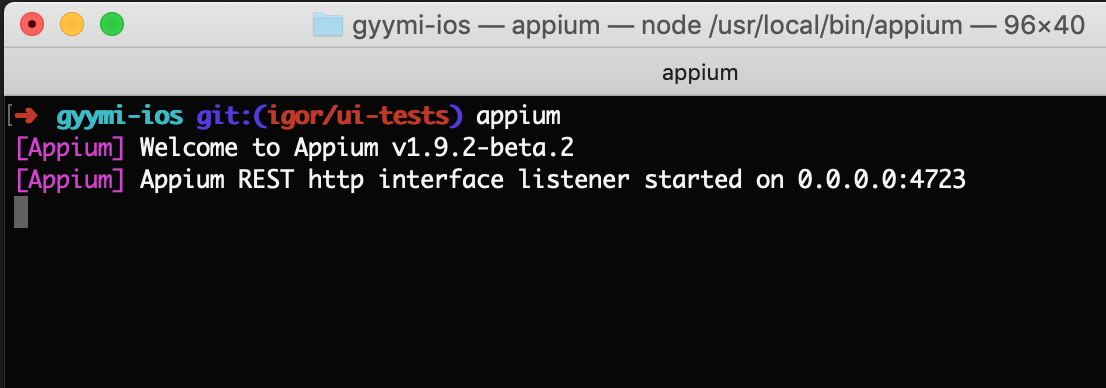
\includegraphics[width=0.8\textwidth]{pfc/figuras/appium-cli.png}
    \caption{CLI do Appium}
    \label{fig:appium-cli}
\end{figure}

\begin{figure}[H]
    \centering
    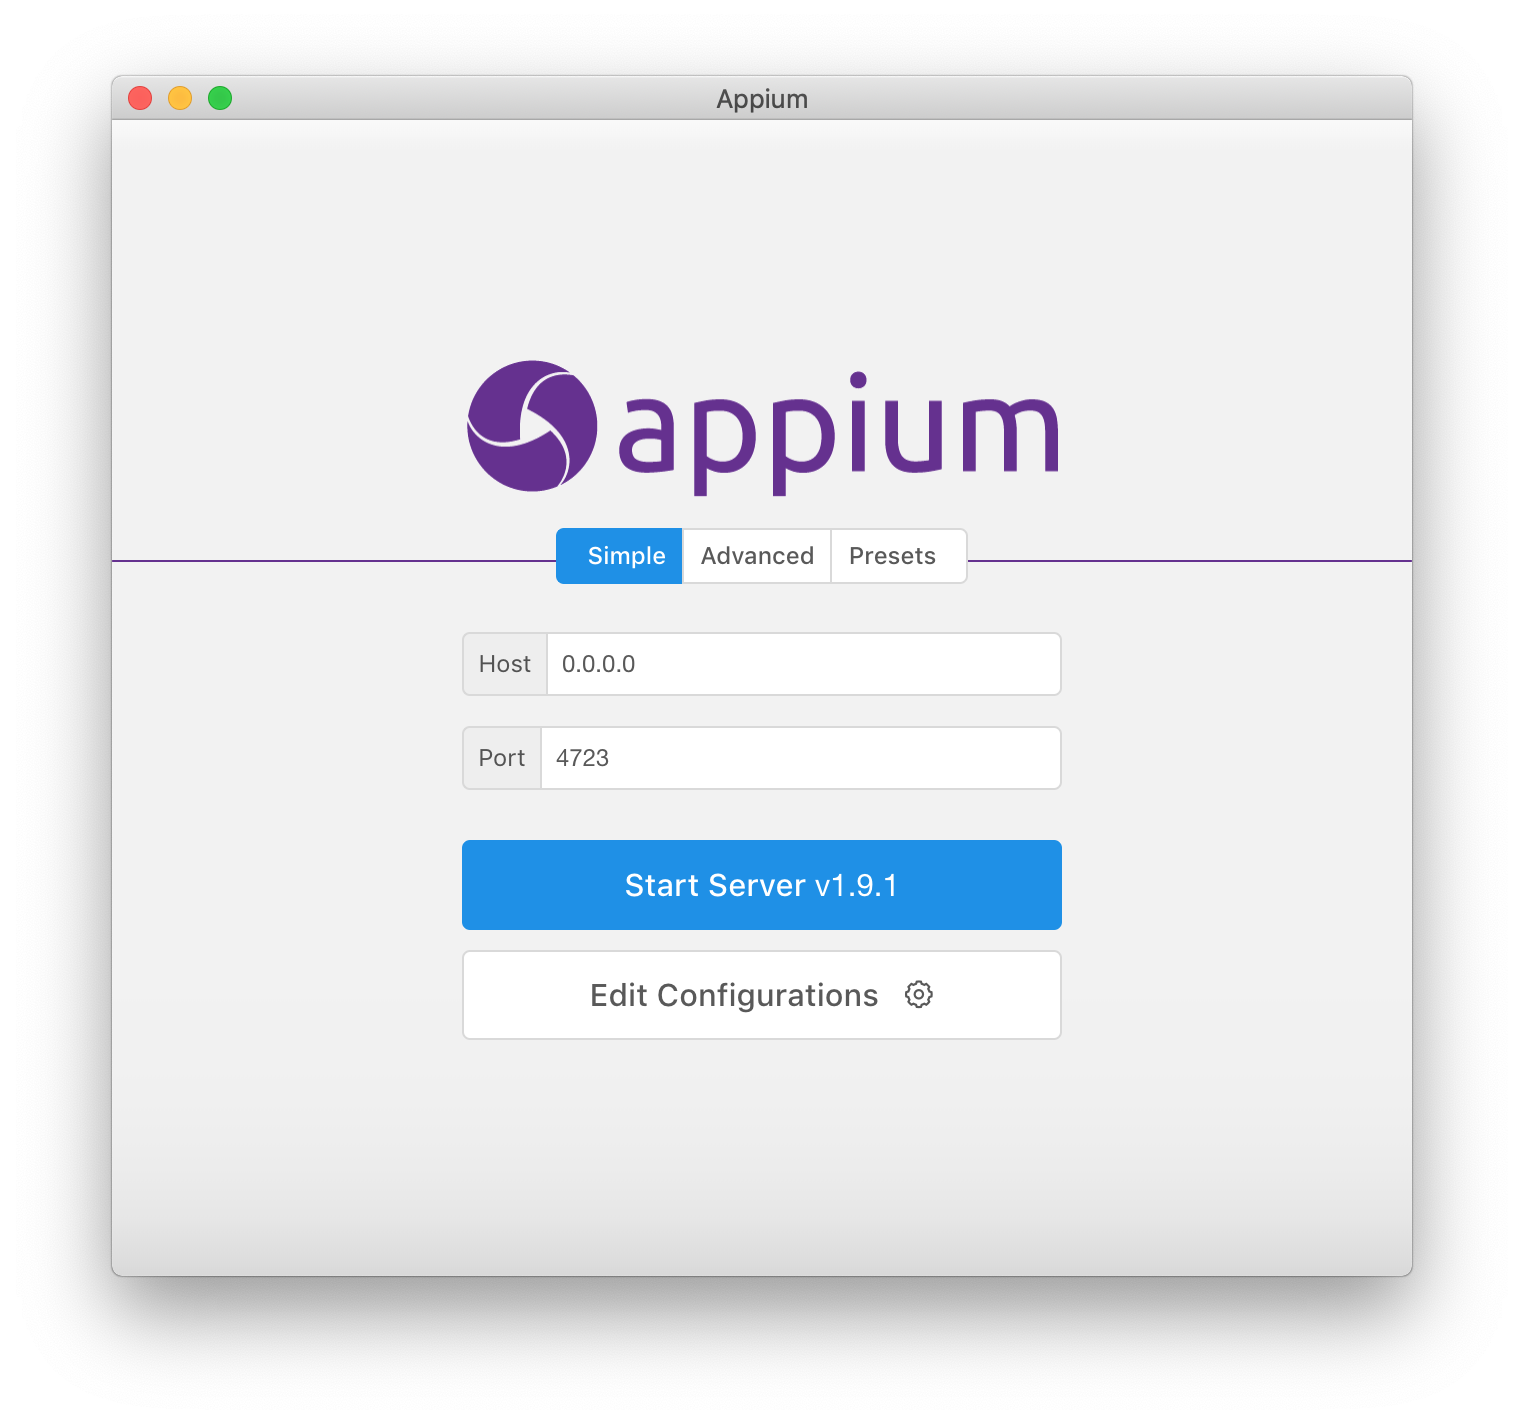
\includegraphics[width=0.8\textwidth]{pfc/figuras/appium-desktop.png}
    \caption{GUI do Appium}
    \label{fig:appium-desktop}
\end{figure}

\begin{figure}[H]
    \centering
    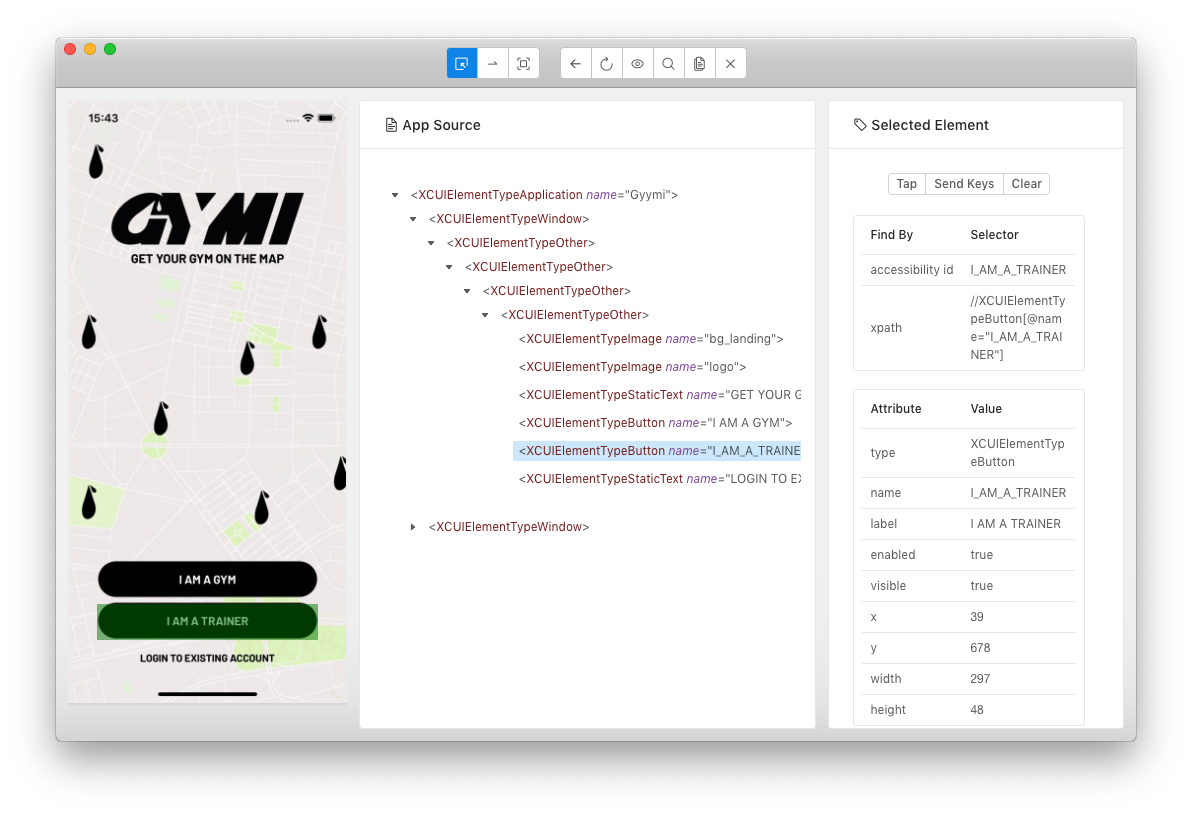
\includegraphics[width=0.8\textwidth]{pfc/figuras/appium-desktop-inspector.png}
    \caption{Ferramenta de inspeção do Appium}
    \label{fig:appium-desktop-inspector}
\end{figure}

\subsection{EarlGrey}
A configuração do EarlGrey requer menos passos, já que sua utilização é feita pelo Xcode. Primeiramente, um novo objeto de projeto (\textit{target} em inglês) dentro do Xcode foi criado para isolar o código de testes e o referente à aplicação. Assim, a compilação do código dos testes e da aplicação dá-se de forma separada, bem como a configuração de dependências para os dois casos. Por último, o EarlGrey é adicionado como dependência do código dos testes automatizados.

\section{Casos de Teste}

\subsection{Estratégia de Implementação}
A implementação dos testes seguiu o paradigma de programação orientado a objetos. A escolha da abordagem foi feita pelo fato do código do aplicativo também utilizar o paradigma como estrutura. A Figura \ref{fig:class-diagram-tests} apresenta o diagrama de classes para os casos de teste. Uma classe base foi criada para implementar os métodos comuns aos casos de teste, como chamadas para iniciar e encerrar gravações de vídeo, tirar fotos da tela e preencher campos de texto. Além disso, a classe base contém uma propriedade que referencia um objeto de geração de conteúdo (implementado por bibliotecas de terceiros), o qual simula a entrada de dados de um usuário real. Em seguida, uma classe foi criada para cada cenário de teste, contendo os métodos específicos para cada caso.

O código segue uma abordagem declarativa, isto é, são criadas camadas de abstrações através de funções que representam o que é realizado no teste. A estratégia tem o objetivo de possibilitar o reuso de código, aumentar a legibilidade e permitir que pessoas que não tem contato com as linguagens e ferramentas compreendam o que o código de teste realiza.

\begin{figure}[H]
    \centering
    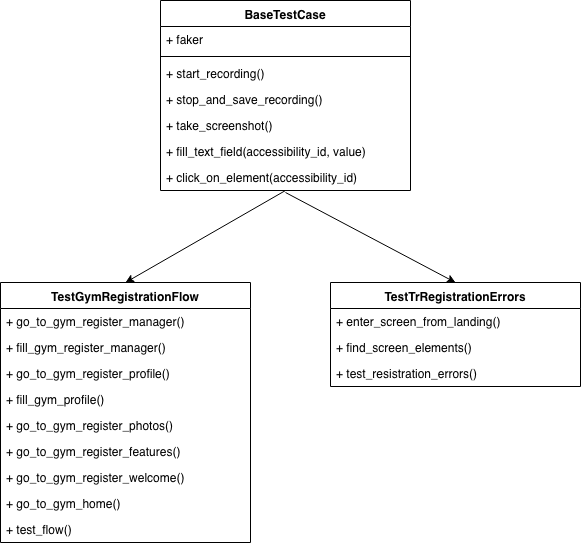
\includegraphics[width=0.8\textwidth]{pfc/figuras/class-diagram-tests.png}
    \caption{Diagrama de classes para os casos de teste}
    \label{fig:class-diagram-tests}
\end{figure}

\subsection{Fluxo de Cadastro das Academias}
Este primeiro caso tem como objetivo testar o fluxo de cadastro de academias no aplicativo. A sequência tem início na tela de entrada do aplicativo (Figura \ref{fig:landing}) e encerra-se ao final do cadastro (Figura \ref{fig:gym-welcome}). O teste tem sucesso se todas as etapas do cadastro são concluídas, ou seja, da perspectiva da interface gráfica, todas as telas de cadastro devem ser visualizadas. Garantir que este fluxo funcione da maneira esperada é de fundamental importância, uma vez que as principais interações no aplicativo ocorrem em torno da entidade da academia.

A implementação deste cenário de teste foi realizada no Appium e no EarlGrey. A Figura \ref{fig:test-flow} ilustra o trecho de código em que o método principal do caso de teste é chamado em ambas as ferramentas. Nota-se uma grande semelhança nos dois códigos implementados para cada uma das ferramentas, em razão da estratégia de código declarativo.

As Figuras \ref{fig:fill-gym-appium} e \ref{fig:fill-gym-earlgrey} apresentam detalhes do código de uma dos métodos da classe do caso de teste. O método é responsável por enviar comandos para simular a interação de um usuário com a interface gráfica, como clicar em botões e preencher campos de texto. O exemplo ilustra o caso do preenchimento da tela de cadastro do perfil da academia (Figura \ref{fig:register-gym-info}).

\begin{figure}[H]
	\centering
    \begin{subfigure}[b]{0.5\textwidth}
        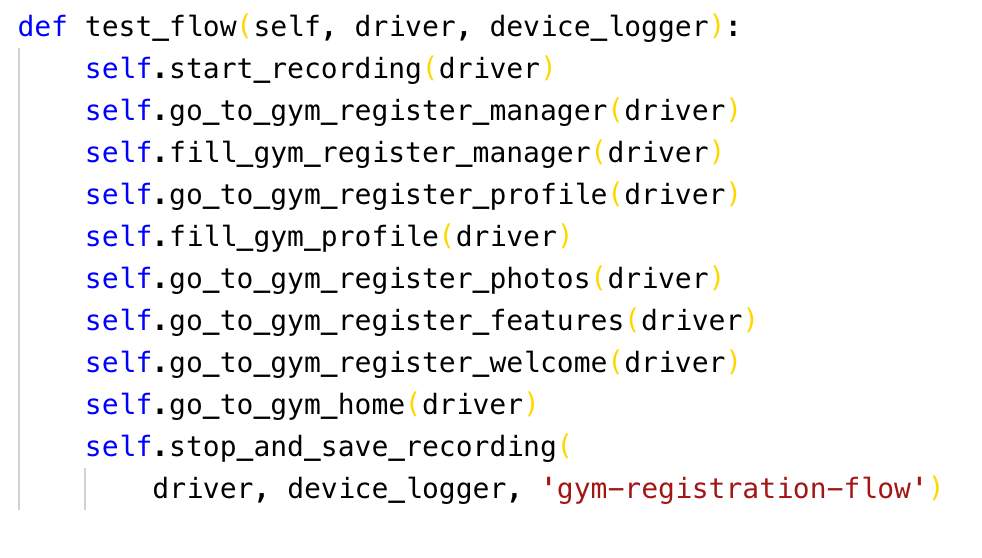
\includegraphics[width=\textwidth]{pfc/figuras/test-flow-appium.png}
        \caption{Appium}
        \label{fig:test-flow-appium}
    \end{subfigure}
    ~
	\begin{subfigure}[b]{0.3\textwidth}
        \includegraphics[width=\textwidth]{pfc/figuras/test-flow-earlgrey.png}
        \caption{EarlGrey}
        \label{fig:test-flow-earlgrey}
    \end{subfigure}
    ~
    \caption{Funções de teste do fluxo de cadastro das academias}
    \label{fig:test-flow}
\end{figure}

\begin{figure}[H]
    \centering
    \includegraphics[width=0.8\textwidth]{pfc/figuras/fill-gym-appium.png}
    \caption{Detalhe de implementação de um método do caso de teste que realiza os comandos para interação com a interface gráfica - Appium}
    \label{fig:fill-gym-appium}
\end{figure}

\begin{figure}[H]
    \centering
    \includegraphics[width=0.8\textwidth]{pfc/figuras/fill-gym-earlgrey.png}
    \caption{Detalhe de implementação de um método do caso de teste que realiza os comandos para interação com a interface gráfica - EarlGrey}
    \label{fig:fill-gym-earlgrey}
\end{figure}

\subsection{Erros de Cadastro do Treinador}
Este caso tem como objetivo testar as mensagens (Figura \ref{fig:error-messages-test}) e estados de erro (Figura \ref{fig:error-states-test}) no preenchimento das informações de usuário do treinador (Figura \ref{fig:register-trainer-info}). O teste tem sucesso se as mensagens correspondem às esperadas para cada caso de erro.

A implementação deste caso foi feita de forma exaustiva, ou seja, todas as combinações possíveis de entradas de campo de texto foram testadas, considerando duas opções para cada entrada: válida ou inválida. Como exemplo, o campo de e-mail teve a entrada "igor@jungledevs.com" considerada válida e a entrada "invalidemail", inválida.

A implementação deste cenário de teste foi realizada somente no Appium. O uso do EarlGrey para este caso foi julgado desnecessário para o estudo, uma vez que o primeiro caso já indicou que a implementação seria semelhante e que informações suficientes para o comparativo entre as ferramentas já haviam sido coletadas. Além disso, a execução do caso de teste mostrou-se demasiadamente lenta, pelo fato de ser exaustiva.

\begin{figure}[H]
	\centering
    \begin{subfigure}[b]{0.3\textwidth}
        \includegraphics[width=\textwidth]{pfc/figuras/email-not-valid.png}
        \caption{E-mail inválido}
        \label{fig:email-not-valid}
    \end{subfigure}
    ~
	\begin{subfigure}[b]{0.3\textwidth}
        \includegraphics[width=\textwidth]{pfc/figuras/password-not-valid.png}
        \caption{Senha inválida}
        \label{fig:password-not-valid}
    \end{subfigure}
    ~
    \begin{subfigure}[b]{0.3\textwidth}
        \includegraphics[width=\textwidth]{pfc/figuras/fields-empty.png}
        \caption{Campo nulo}
        \label{fig:empty-fields}
    \end{subfigure}
    ~
    \caption{Mensagens de erro testadas no cadastro de usuário}
    \label{fig:error-messages-test}
\end{figure}

\begin{figure}[H]
	\centering
    \begin{subfigure}[b]{0.4\textwidth}
        \includegraphics[width=\textwidth]{pfc/figuras/email-not-valid-field.png}
        \caption{Email inválido}
        \label{fig:email-not-valid-field}
    \end{subfigure}
    ~
	\begin{subfigure}[b]{0.4\textwidth}
        \includegraphics[width=\textwidth]{pfc/figuras/phone-not-valid-field.png}
        \caption{Número telefônico inválido}
        \label{fig:phone-not-valid-field}
    \end{subfigure}
    ~
    \caption{Estados de erro testados no cadastro de usuário}
    \label{fig:error-states-test}
\end{figure}

\section{Dificuldades e Limitações do Estudo}
A maior dificuldade de implementação encontrada foi o setup das ferramentas, em particular do Appium. Esta etapa demandou uma porção de tempo considerável em relação ao total despendido para o estudo. A dificuldade foi decorrente da inexperiência da realização do processo pelos membros da empresa e pelo autor. O Appium exigiu um esforço extra por se tratar de uma ferramenta externa ao ambiente de desenvolvimento iOS. Para configurar a ferramenta, foi necessária a instalação de componentes externos de software (como a CLI e GUI do Appium), a instalação de bibliotecas no Python e configuração de integração entre o simulador de dispositivos do Xcode e o servidor web do Appium.

A segunda dificuldade encontrada na condução do estudo foi a identificação de causas de erro na execução dos testes, particularmente no Appium novamente. As mensagens de erro do Appium são mais verbosas que as mensagens do EarlGrey (ver comparação na Figura \ref{fig:error-test-tools}), o que dificulta a identificação da causa do erro.

\begin{figure}[H]
	\centering
    \begin{subfigure}[b]{0.4\textwidth}
        \includegraphics[width=\textwidth]{pfc/figuras/error-appium.png}
        \caption{Erros no Appium}
        \label{fig:error-appium}
    \end{subfigure}
    ~
	\begin{subfigure}[b]{0.4\textwidth}
        \includegraphics[width=\textwidth]{pfc/figuras/error-earlgrey.png}
        \caption{Erros no EarlGrey}
        \label{fig:error-earlgrey}
    \end{subfigure}
    ~
    \caption{Mensagens de error durante a execução dos testes}
    \label{fig:error-test-tools}
\end{figure}

O estudo esteve limitado a testes no aplicativo iOS, excluindo-se a plataforma Android. O autor não esteve envolvido no desenvolvimento do aplicativo para o sistema Android e, em decorrência deste fator, não foi possível aplicar os testes à plataforma por limitações de tempo. Esta restrição influencia a comparação entre as ferramentas, uma vez que uma dos benefícios do Appium é o suporte à múltiplas plataformas.

\chapter{Resultados} \label{cap:results}
Neste capítulo são apresentados os resultados obtidos do trabalho desenvolvido. Primeiramente, os resultados de negócio envolvidos na implementação da aplicação são apresentados. Em seguida, uma comparação das ferramentas de teste automatizado é feita. Por último, são discutidos os resultados obtidos do ponto de vista da empresa em que este projeto esteve inserido.

\section{Versão Piloto}
\subsection{Uso do Aplicativo}
O desenvolvimento do aplicativo para o sistema iOS, apresentado neste trabalho, culminou no lançamento da sua versão piloto. Esta versão consiste na primeira etapa de lançamentos do produto e tem como objetivo a validação da ideia. O aplicativo piloto foi avaliado por um grupo seleto de academias e treinadores, localizados em Sydney.

A Figura \ref{fig:pilot-use} ilustra a utilização da versão piloto do aplicativo, com dados coletados da ferramenta Fabric. O gráfico mostra o número de usuários ativos diariamente desde o lançamento do piloto. O eixo horizontal representa a evolução temporal em dias, enquanto o eixo vertical contém o número total de usuários diários. O primeiro pico (entre os dias 10 e 28 de outubro) corresponde a distribuição de um incremento da versão piloto, ultrapassando o número de 10 usuários. O segundo e o terceiro picos (entre os dias 4 e 11 de novembro) dizem respeito a uma nova versão de incremento do piloto, com o convite de mais parceiros para o teste do aplicativo. Totalizando 19 usuários utilizando a aplicação.

\begin{figure}[H]
    \centering
    \includegraphics[width=\textwidth]{pfc/figuras/pilot-use.png}
    \caption{Uso diário da versão piloto do aplicativo}
    \label{fig:pilot-use}
\end{figure}

\subsection{Desenvolvimento do Produto}
O resultado da implementação da aplicação, no período contemplado neste PFC de aproximadamente 4 meses, contribuíram para grandes avanços no desenvolvimento do produto. A versão atual do aplicativo para o sistema iOS totaliza 33 telas principais de interação com o usuário (Figura \ref{fig:all-screens}). Estas interfaces permitem que os seguintes fluxos de atividade sejam realizados pelos usuários finais do produto:
\begin{itemize}
    \item Cadastro de academias;
    \item Cadastro de treinadores;
    \item Construção de agenda semanal de blocos para locação nas academias;
    \item Acompanhamento diário de sessões de treino agendadas nas academias;
    \item Visualização de dados semanais das academias em dashboard;
    \item Visualização e edição de perfil das academias;
    \item Busca por academias disponíveis em mapa dinâmico;
    \item Adição de academias à seleção de favoritos;
    \item Visualização de agenda diária dos treinadores;
    \item Cancelamento e avaliação de sessões de treino;
    \item Visualização e edição de perfil de treinador;
    \item Visualização de dados semanais dos treinadores em dashboard;
    \item Visualização de disponibilidade diária de blocos de academias através de calendário;
    \item Agendamento de sessão de treino.
\end{itemize}
\begin{figure}[H]
	\centering
    \includegraphics[width=0.14\textwidth]{pfc/figuras/landing.png}
    \includegraphics[width=0.14\textwidth]{pfc/figuras/login.png}
    \includegraphics[width=0.14\textwidth]{pfc/figuras/register-manager.png}
    \includegraphics[width=0.14\textwidth]{pfc/figuras/register-gym-info.png}
    \includegraphics[width=0.14\textwidth]{pfc/figuras/register-gym-photos.png}
    \includegraphics[width=0.14\textwidth]{pfc/figuras/register-gym-amenities.png}
    \includegraphics[width=0.14\textwidth]{pfc/figuras/gym-welcome.png}
    \includegraphics[width=0.14\textwidth]{pfc/figuras/bank-details.png}
    \includegraphics[width=0.14\textwidth]{pfc/figuras/gym-block-structure.png}
    \includegraphics[width=0.14\textwidth]{pfc/figuras/gym-add-block.png}
    \includegraphics[width=0.14\textwidth]{pfc/figuras/gym-booking-calendar.png}
    \includegraphics[width=0.14\textwidth]{pfc/figuras/gym-booking-detail.png}
    \includegraphics[width=0.14\textwidth]{pfc/figuras/gym-dashboard.png}
    \includegraphics[width=0.14\textwidth]{pfc/figuras/gym-profile.png}
    \includegraphics[width=0.14\textwidth]{pfc/figuras/register-trainer.png}
    \includegraphics[width=0.14\textwidth]{pfc/figuras/register-trainer-verification.png}
    \includegraphics[width=0.14\textwidth]{pfc/figuras/tr-congratulations.png}
    \includegraphics[width=0.14\textwidth]{pfc/figuras/tr-register-profile-1.png}
    \includegraphics[width=0.14\textwidth]{pfc/figuras/tr-gym-profile-2.png}
    \includegraphics[width=0.14\textwidth]{pfc/figuras/tr-register-profile-3.png}
    \includegraphics[width=0.14\textwidth]{pfc/figuras/tr-home-map.png}
    \includegraphics[width=0.14\textwidth]{pfc/figuras/tr-favorite.png}
    \includegraphics[width=0.14\textwidth]{pfc/figuras/tr-my-gyms.png}
    \includegraphics[width=0.14\textwidth]{pfc/figuras/tr-calendar.png}
    \includegraphics[width=0.14\textwidth]{pfc/figuras/tr-profile.png}
    \includegraphics[width=0.14\textwidth]{pfc/figuras/tr-dashboard.png}
    \includegraphics[width=0.14\textwidth]{pfc/figuras/add-card.png}
    \includegraphics[width=0.14\textwidth]{pfc/figuras/manage-cards.png}
    \includegraphics[width=0.14\textwidth]{pfc/figuras/tr-gym-profile-2.png}
    \includegraphics[width=0.14\textwidth]{pfc/figuras/tr-availability-2.png}
    \includegraphics[width=0.14\textwidth]{pfc/figuras/tr-new-booking.png}
    \includegraphics[width=0.14\textwidth]{pfc/figuras/tr-booking-payment.png}
    \includegraphics[width=0.14\textwidth]{pfc/figuras/tr-booking-confirmed.png}
    \caption{Todas as telas desenvolvidas para a versão piloto}
    \label{fig:all-screens}
\end{figure}

\section{Validação do Programa de Capacitação da Empresa}
O presente trabalho esteve inserido na empresa Jungle Devs como parte do programa de capacitação do autor. O programa de capacitação \textit{Academy} não havia sido concluído por nenhuma pessoa anteriormente. Portanto, um dos resultados obtidos por este PFC para a empresa é a validação do programa.

A proposta de conclusão de um projeto de aplicação prática real, em conjunto com um time de engenharia de software, foi efetuada com sucesso. O projeto do aplicativo Gyymi para o sistema iOS se mostrou eficaz para a capacitação do autor em projetos de aplicações \textit{mobile}. Isso se deve ao fato do aplicativo contemplar a maioria das funcionalidades recorrentes em aplicativos em produção no mercado, como cadastro e autenticação de usuários, navegação customizada por múltiplas telas e integração com sistemas de software terceiros.

Além de validar a etapa final do programa \textit{Academy}, na qual o projeto do aplicativo esteve inserido, o trabalho revelou bons resultados no que diz respeito às etapas anteriores. Esta afirmação é justificada a partir da análise da contribuição prática do autor para o projeto. A partir dos dados disponíveis no repositório do código fonte da aplicação (ver Figura \ref{fig:github-stats}), é possível concluir que o autor teve contribuições significativas desde o começo do projeto. Os dados indicam a contribuição do autor em $70\%$ das linhas de código modificadas durante o projeto, totalizando $55408$ alterações. Além disso, o autor teve contribuição em $74\%$ dos incrementos de versão do código (\textit{commits}), totalizando $699$ mensagens de incremento salvas. Assim, é possível concluir que as etapas iniciais do programa de capacitação foram efetivas para a aprendizagem de conceitos práticos de projeto.
\begin{figure}[H]
    \centering
    \includegraphics[width=\textwidth]{pfc/figuras/github-stats.png}
    \caption{Dados de contribuição no projeto do aplicativo iOS por membro do time}
    \label{fig:github-stats}
\end{figure}

\section{Testes Automatizados}


% ----------------------------------------------------------
% Finaliza a parte no bookmark do PDF
% para que se inicie o bookmark na raiz
% e adiciona espaço de parte no Sumário
% ----------------------------------------------------------
\phantompart

% ----------------------------------------------------------
% ELEMENTOS PÓS-TEXTUAIS
% ----------------------------------------------------------
\postextual
\bibliography{referencias}
% \glossary
% 
% ----------------------------------------------------------
% Apêndices
% ----------------------------------------------------------

% ---
% Inicia os apêndices
% ---
\begin{apendicesenv}

% Imprime uma página indicando o início dos apêndices
\partapendices

% ----------------------------------------------------------
\chapter{Quisque libero justo}
% ----------------------------------------------------------

\lipsum[50]

% ----------------------------------------------------------
\chapter{Nullam elementum urna vel imperdiet sodales elit ipsum pharetra ligula
ac pretium ante justo a nulla curabitur tristique arcu eu metus}
% ----------------------------------------------------------
\lipsum[55-57]

\end{apendicesenv}
% ---
% % ---
% Anexos
% ---

\begin{anexosenv}

% Imprime uma página indicando o início dos anexos
\partanexos

\chapter{Morbi ultrices rutrum lorem.}
% \lipsum[30]

\chapter{Cras non urna sed feugiat cum sociis natoque penatibus et magnis dis
parturient montes nascetur ridiculus mus}
% \lipsum[31]

\chapter{Fusce facilisis lacinia dui}
% \lipsum[32]

\end{anexosenv}

%---------------------------------------------------------------------
% INDICE REMISSIVO
%---------------------------------------------------------------------
\phantompart
\printindex

\end{document}
